Addressing the research problems and corresponding questions ultimately means ensuring the induced agility enablers. Accordingly, we first present a modeling strategy and then propose a method to provide such enablers.

We model agility enablers as QAs. Quality levels according to domain requirements are monitored to identify the need for system's adaptation to keep the C2 Agility. Furthermore, our approach has to deal with multiple QAs, since the domain works with more than one quality attribute (QA) during system execution. System adaptation must occur according to the effects of all measured attributes. 

Assuming this modeling strategy and to deliver the agility enablers, we follow the dimensions of realizing multiple QAs in self-adaptive systems defined by~\textit{Mahdavi-Hezavehi et al.}~\cite{SAS_001}. Accordingly, we propose the process shown in Figure~\ref{process}. The first step, QA Specification, defines QAs of interest as goals of the system's adaptation. All domain requirements are analyzed to define the desired levels for these attributes. Next, the second step, QA Monitoring and Treatment, defines the aspects to build a strategy to monitor and to treat multiple QAs sets. The third step, QA Handling, specifies the self-adaptation mechanism that deals with the QAs.   In our case, this mechanism amounts to multiple feedback loops, acting in layers, within the members in the C2 System. Finally, QA Guarantees defines mechanism to validate the measurements and results obtained indicating that the system satisfies all quality requirements.

% TODO please fix in the figure: "QA Handling" -> "QA Handling and Treatment" 
%  "QA Handling and Treatment" -> "QA Handling"
% TODO in the figure, we should have MDSPL label a horizontal square bracket spanning
% both "QA Monitoring and Treatment" and "QA Handling"
%%%%%% OK %%%%%%%%%%
\begin{figure}[h]
\centering
\scalebox{.8}{


\tikzset{every picture/.style={line width=0.75pt}} %set default line width to 0.75pt        

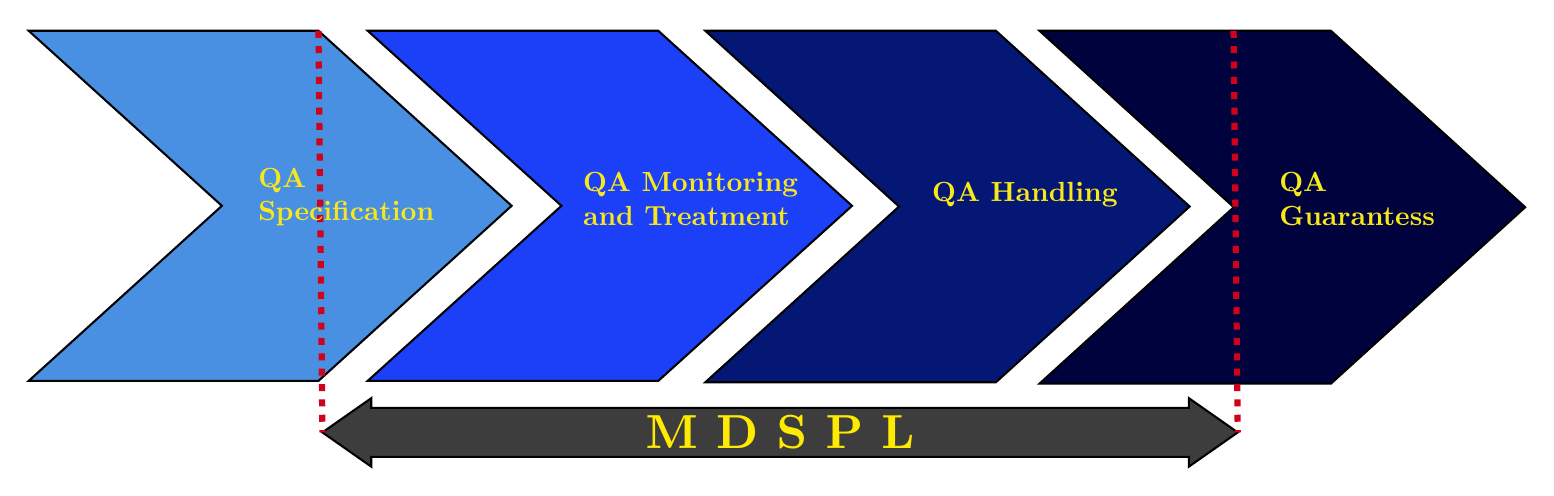
\begin{tikzpicture}[x=0.75pt,y=0.75pt,yscale=-1,xscale=1]
%uncomment if require: \path (0,268); %set diagram left start at 0, and has height of 268

%Chevron Arrow [id:dp7998116230156174] 
\draw  [fill={rgb, 255:red, 28; green, 64; blue, 248 }  ,fill opacity=1 ] (180.33,40) -- (320.33,40) -- (413.67,124.33) -- (320.33,208.67) -- (180.33,208.67) -- (273.67,124.33) -- cycle ;
%Chevron Arrow [id:dp17326121534239214] 
\draw  [fill={rgb, 255:red, 74; green, 144; blue, 226 }  ,fill opacity=1 ] (17,40) -- (156.6,40) -- (249.67,124.33) -- (156.6,208.67) -- (17,208.67) -- (110.07,124.33) -- cycle ;
%Chevron Arrow [id:dp2103753298875829] 
\draw  [fill={rgb, 255:red, 5; green, 23; blue, 117 }  ,fill opacity=1 ] (343,40) -- (483,40) -- (576.33,124.67) -- (483,209.33) -- (343,209.33) -- (436.33,124.67) -- cycle ;
%Chevron Arrow [id:dp7759460284870137] 
\draw  [fill={rgb, 255:red, 0; green, 2; blue, 61 }  ,fill opacity=1 ] (504,40) -- (644.4,40) -- (738,125) -- (644.4,210) -- (504,210) -- (597.6,125) -- cycle ;
%Left Right Arrow [id:dp5098219629430656] 
\draw  [fill={rgb, 255:red, 7; green, 7; blue, 7 }  ,fill opacity=0.78 ] (158.5,233.5) -- (182.05,217) -- (182.05,221.71) -- (575.95,221.71) -- (575.95,217) -- (599.5,233.5) -- (575.95,250) -- (575.95,245.29) -- (182.05,245.29) -- (182.05,250) -- cycle ;
%Straight Lines [id:da7722048533467026] 
\draw [color={rgb, 255:red, 208; green, 2; blue, 27 }  ,draw opacity=1 ][line width=2.25]  [dash pattern={on 2.53pt off 3.02pt}]  (156.6,40) -- (158.5,233.5) ;


%Straight Lines [id:da37299757229242914] 
\draw [color={rgb, 255:red, 208; green, 2; blue, 27 }  ,draw opacity=1 ][line width=2.25]  [dash pattern={on 2.53pt off 3.02pt}]  (597.5,40) -- (599.5,233.5) ;



% Text Node
\draw (170,120) node [color={rgb, 255:red, 248; green, 231; blue, 28 }  ,opacity=1 ] [align=left] {\textbf{QA}\\\textbf{Specification}};
% Text Node
\draw (336,121) node [color={rgb, 255:red, 248; green, 231; blue, 28 }  ,opacity=1 ] [align=left] {\textbf{QA Monitoring}\\\textbf{and Treatment}};
% Text Node
\draw (657,121) node  [align=left] {\textbf{\textcolor[rgb]{0.97,0.91,0.11}{QA }}\\\textbf{\textcolor[rgb]{0.97,0.91,0.11}{Guarantess}}};
% Text Node
\draw (497,119) node  [align=left] {\textbf{\textcolor[rgb]{0.97,0.91,0.11}{QA Handling}}};
% Text Node
\draw (379,233.5) node [scale=1.7280000000000002,color={rgb, 255:red, 255; green, 235; blue, 0 }  ,opacity=1 ] [align=left] {\textbf{M D S P L}};


\end{tikzpicture}}
\label{process}
\caption{Process to provide agility guided by QA. MDSPL is the realization.}
\end{figure}
  

%%% COMMENTED BY THE ADVISOR %%%%
%Figure \ref{qas} shows the dimensions defined in \cite{qa01} presented as a flow with four steps that can be applied to identify, to monitor and to adjust multiple QAs. We adapted the list of quality categories to work as a loop due to the possibility of goal changes occurs during the execution under circumstances change. With these changes, there are impacts on the QAs and between QAs. These dimensions are focused on QAs during and after adaptation process of a SAS.

%\begin{figure}[h]
%\centering
%\scalebox{.6}{


\tikzset{every picture/.style={line width=0.75pt}} %set default line width to 0.75pt        

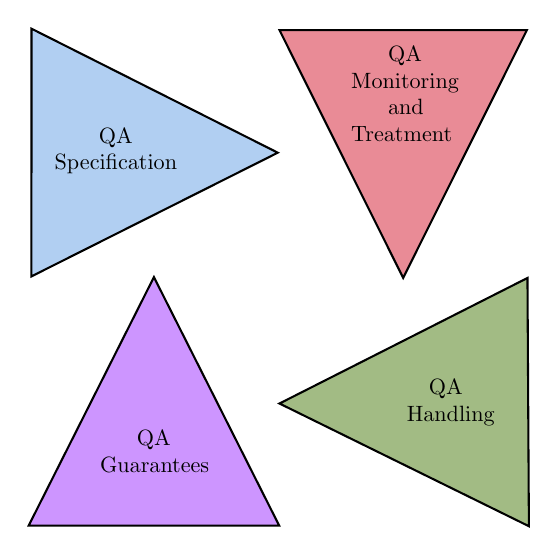
\begin{tikzpicture}[x=0.75pt,y=0.75pt,yscale=-1,xscale=1]
%uncomment if require: \path (0,262); %set diagram left start at 0, and has height of 262

%Flowchart: Extract [id:dp5939698678534469] 
\draw  [fill={rgb, 255:red, 74; green, 144; blue, 226 }  ,fill opacity=0.43 ] (131,70.03) -- (12.3,129.64) -- (12.36,10.3) -- cycle ;
%Flowchart: Merge [id:dp5767066916635984] 
\draw  [fill={rgb, 255:red, 208; green, 2; blue, 27 }  ,fill opacity=0.46 ] (131.83,11) -- (251,11) -- (191.42,130.33) -- cycle ;
%Flowchart: Extract [id:dp6600751137454604] 
\draw  [fill={rgb, 255:red, 65; green, 117; blue, 5 }  ,fill opacity=0.49 ] (131.82,190.88) -- (251.3,130.39) -- (251.99,249.99) -- cycle ;
%Flowchart: Extract [id:dp5337732612018415] 
\draw  [fill={rgb, 255:red, 144; green, 19; blue, 254 }  ,fill opacity=0.45 ] (71.33,130) -- (131.67,249.67) -- (11,249.67) -- cycle ;

% Text Node
\draw (53,69.33) node [scale=0.8] [align=left] { \ \ \ \ \ \ QA \\Specification};
% Text Node
\draw (192.33,41.67) node [scale=0.8] [align=left] { \ \ \ \ \ QA\\Monitoring \\ \ \ \ \ \ and \\Treatment};
% Text Node
\draw (214.33,190.33) node [scale=0.8] [align=left] { \ \ \ QA \\Handling};
% Text Node
\draw (71.67,214) node [scale=0.8] [align=left] { \ \ \ \ \ QA\\Guarantees};


\end{tikzpicture}
}
%\label{qas}
%\caption{Dimensions for realizing multiple QA in SAS (Adapted from \cite{qa01})}
%\end{figure}

%The flow starts from QA Specification where the QAs, mapped as goals, are identified and their priority are adjusted according to changes performed in one or more quality attributes or in the circumstances. At this moment, the QA will be treated during system adaptation according to its importance and its role as a system goal.

%On the second dimension, QA Monitoring and Treating, we define which QA set will be monitored and treated and it guides the system adaptation process. In this dimension, the QAs treatment in SAS, their preference and priority are worked to deal with collateral effects of some quality violations.

%Dealing with the SAS mechanisms that treat QAs, the QA Handling involves different strategies to modelling QA sets and permits to have mechanisms regarding types and formats in adaptation. Finally, the QA Guarantees assures the system capability to keep the QAs levels within acceptable range.



\subsection{Multi Dynamic Software Product Line (MDSPL) }

%%% COMMENTED BY THE ADVISOR %%%%
%Our modelling is based on Self-Adaptive Systems (SAS) architecture using controllers to monitor stimulus, e.g., feedback loops, capable to monitor, analyse and adapt the system components according to context changes. DSPL is an approach to implement this architecture and it is based on commonalities and variabilities to generate all different products.

To realize the previously presented process for achieving agility enables, we further reduce such enablers to two fundamental requirements: configuration and coordination of members in the team comprising the C2 System. Figure \ref{c2a2} trace such requirements to agility dimensions and the enablers listed in Table~\ref{table:table06} that are related with our RQs. 

\begin{figure}[h]
\centering
\label{c2a2}
\scalebox{.7}{


\tikzset{every picture/.style={line width=0.75pt}} %set default line width to 0.75pt        

\begin{tikzpicture}[x=0.75pt,y=0.75pt,yscale=-1,xscale=1]
%uncomment if require: \path (0,429); %set diagram left start at 0, and has height of 429

%Shape: Regular Polygon [id:dp7067589168266406] 
\draw  [dash pattern={on 1.69pt off 2.76pt}][line width=1.5]  (426.47,162.71) -- (354.06,391.95) -- (113.66,393.92) -- (37.5,165.9) -- (230.82,23.01) -- cycle ;
%Flowchart: Terminator [id:dp14433560438481596] 
\draw   (95.3,208) -- (200.7,208) .. controls (214.4,208) and (225.5,216.95) .. (225.5,228) .. controls (225.5,239.05) and (214.4,248) .. (200.7,248) -- (95.3,248) .. controls (81.6,248) and (70.5,239.05) .. (70.5,228) .. controls (70.5,216.95) and (81.6,208) .. (95.3,208) -- cycle ;
%Flowchart: Terminator [id:dp6207310578852377] 
\draw   (271.08,208) -- (373.42,208) .. controls (386.72,208) and (397.5,216.95) .. (397.5,228) .. controls (397.5,239.05) and (386.72,248) .. (373.42,248) -- (271.08,248) .. controls (257.78,248) and (247,239.05) .. (247,228) .. controls (247,216.95) and (257.78,208) .. (271.08,208) -- cycle ;
%Shape: Cross [id:dp691351701136063] 
\draw  [color={rgb, 255:red, 74; green, 144; blue, 226 }  ,draw opacity=1 ][fill={rgb, 255:red, 74; green, 144; blue, 226 }  ,fill opacity=1 ] (234.1,174) -- (237.57,174) -- (237.57,181.93) -- (245.5,181.93) -- (245.5,185.65) -- (237.57,185.65) -- (237.57,193.58) -- (234.1,193.58) -- (234.1,185.65) -- (226.17,185.65) -- (226.17,181.93) -- (234.1,181.93) -- cycle ;
%Shape: Cube [id:dp0230534183880875] 
\draw  [blur shadow={shadow xshift=2.25pt,shadow yshift=-2.25pt, shadow blur radius=3.75pt, shadow blur steps=5 ,shadow opacity=100}] (170.5,90.1) -- (184.6,76) -- (286.5,76) -- (286.5,108.9) -- (272.4,123) -- (170.5,123) -- cycle ; \draw  [blur shadow={shadow xshift=2.25pt,shadow yshift=-2.25pt, shadow blur radius=3.75pt, shadow blur steps=5 ,shadow opacity=100}] (286.5,76) -- (272.4,90.1) -- (170.5,90.1) ; \draw  [blur shadow={shadow xshift=2.25pt,shadow yshift=-2.25pt, shadow blur radius=3.75pt, shadow blur steps=5 ,shadow opacity=100}] (272.4,90.1) -- (272.4,123) ;
%Shape: Circle [id:dp4505895342746954] 
\draw  [color={rgb, 255:red, 74; green, 144; blue, 226 }  ,draw opacity=1 ] (221.92,183.95) .. controls (221.92,176.28) and (228.13,170.06) .. (235.8,170.06) .. controls (243.47,170.06) and (249.69,176.28) .. (249.69,183.95) .. controls (249.69,191.62) and (243.47,197.83) .. (235.8,197.83) .. controls (228.13,197.83) and (221.92,191.62) .. (221.92,183.95) -- cycle ;
%Curve Lines [id:da06503409897371804] 
\draw [color={rgb, 255:red, 65; green, 117; blue, 5 }  ,draw opacity=1 ][line width=1.5]    (373.42,208) .. controls (351.83,181.4) and (309.12,180.9) .. (259.28,183.7) ;
\draw [shift={(257,183.83)}, rotate = 356.68] [color={rgb, 255:red, 65; green, 117; blue, 5 }  ,draw opacity=1 ][line width=1.5]    (14.21,-6.37) .. controls (9.04,-2.99) and (4.3,-0.87) .. (0,0) .. controls (4.3,0.87) and (9.04,2.99) .. (14.21,6.37)   ;

%Curve Lines [id:da7213073309304452] 
\draw [color={rgb, 255:red, 65; green, 117; blue, 5 }  ,draw opacity=1 ][line width=1.5]    (95.3,208) .. controls (109.29,178.45) and (148.79,181.09) .. (210.82,183.71) ;
\draw [shift={(213.67,183.83)}, rotate = 182.38] [color={rgb, 255:red, 65; green, 117; blue, 5 }  ,draw opacity=1 ][line width=1.5]    (14.21,-6.37) .. controls (9.04,-2.99) and (4.3,-0.87) .. (0,0) .. controls (4.3,0.87) and (9.04,2.99) .. (14.21,6.37)   ;

%Striped Right Arrow [id:dp8375916226786752] 
\draw  [fill={rgb, 255:red, 208; green, 2; blue, 27 }  ,fill opacity=1 ] (225.18,154.11) -- (225.3,143.06) -- (215.82,142.96) -- (234.92,130.54) -- (253.74,143.37) -- (244.26,143.27) -- (244.14,154.32) -- cycle ;\draw  [fill={rgb, 255:red, 208; green, 2; blue, 27 }  ,fill opacity=1 ] (225.1,162) -- (225.12,160.42) -- (244.07,160.63) -- (244.06,162.21) -- cycle ;\draw  [fill={rgb, 255:red, 208; green, 2; blue, 27 }  ,fill opacity=1 ] (225.13,158.84) -- (225.17,155.69) -- (244.13,155.89) -- (244.09,159.05) -- cycle ;
%Curve Lines [id:da6776255511162914] 
\draw [line width=1.5]    (152.5,302) .. controls (140.92,287.52) and (140.51,277.71) .. (139.6,252.77) ;
\draw [shift={(139.5,250)}, rotate = 447.88] [color={rgb, 255:red, 0; green, 0; blue, 0 }  ][line width=1.5]    (14.21,-4.28) .. controls (9.04,-1.82) and (4.3,-0.39) .. (0,0) .. controls (4.3,0.39) and (9.04,1.82) .. (14.21,4.28)   ;

%Curve Lines [id:da8603928726112443] 
\draw [line width=1.5]  [dash pattern={on 5.63pt off 4.5pt}]  (177.5,302) .. controls (203.24,265.37) and (242.7,289.51) .. (298.8,251.18) ;
\draw [shift={(300.5,250)}, rotate = 504.94] [color={rgb, 255:red, 0; green, 0; blue, 0 }  ][line width=1.5]    (14.21,-4.28) .. controls (9.04,-1.82) and (4.3,-0.39) .. (0,0) .. controls (4.3,0.39) and (9.04,1.82) .. (14.21,4.28)   ;

%Curve Lines [id:da34743038227858414] 
\draw [line width=1.5]  [dash pattern={on 5.63pt off 4.5pt}]  (296,335) .. controls (263.99,301.51) and (197.53,303.92) .. (179.3,250.48) ;
\draw [shift={(178.5,248)}, rotate = 433.11] [color={rgb, 255:red, 0; green, 0; blue, 0 }  ][line width=1.5]    (14.21,-4.28) .. controls (9.04,-1.82) and (4.3,-0.39) .. (0,0) .. controls (4.3,0.39) and (9.04,1.82) .. (14.21,4.28)   ;

%Curve Lines [id:da6081182817919902] 
\draw [line width=1.5]    (309,334) .. controls (334.97,307.54) and (320.12,299.33) .. (331.75,254.77) ;
\draw [shift={(332.5,252)}, rotate = 465.46] [color={rgb, 255:red, 0; green, 0; blue, 0 }  ][line width=1.5]    (14.21,-4.28) .. controls (9.04,-1.82) and (4.3,-0.39) .. (0,0) .. controls (4.3,0.39) and (9.04,1.82) .. (14.21,4.28)   ;

%Rounded Rect [id:dp7632161896108657] 
\draw   (97.5,310.2) .. controls (97.5,307.33) and (99.83,305) .. (102.7,305) -- (230.3,305) .. controls (233.17,305) and (235.5,307.33) .. (235.5,310.2) -- (235.5,325.8) .. controls (235.5,328.67) and (233.17,331) .. (230.3,331) -- (102.7,331) .. controls (99.83,331) and (97.5,328.67) .. (97.5,325.8) -- cycle ;
%Flowchart: Alternative Process [id:dp12800150200605298] 
\draw   (228.5,341.03) .. controls (228.5,338.8) and (230.3,337) .. (232.53,337) -- (359.48,337) .. controls (361.7,337) and (363.5,338.8) .. (363.5,341.03) -- (363.5,355.98) .. controls (363.5,358.2) and (361.7,360) .. (359.48,360) -- (232.53,360) .. controls (230.3,360) and (228.5,358.2) .. (228.5,355.98) -- cycle ;

% Text Node
\draw (143,228) node  [align=left] {C2 Approach Agility};
% Text Node
\draw (339,80) node [scale=1.2,color={rgb, 255:red, 208; green, 2; blue, 27 }  ,opacity=1 ,rotate=-36.41] [align=left] {Resilience};
% Text Node
\draw (406,281) node [scale=1.2,color={rgb, 255:red, 208; green, 2; blue, 27 }  ,opacity=1 ,rotate=-288.33] [align=left] {Robustness};
% Text Node
\draw (123,82) node [scale=1.2,color={rgb, 255:red, 208; green, 2; blue, 27 }  ,opacity=1 ,rotate=-323.02] [align=left] {Flexibility};
% Text Node
\draw (235,407) node [scale=1.2,color={rgb, 255:red, 208; green, 2; blue, 27 }  ,opacity=1 ] [align=left] {Adaptability};
% Text Node
\draw (58,284) node [scale=1.2,color={rgb, 255:red, 208; green, 2; blue, 27 }  ,opacity=1 ,rotate=-72.21] [align=left] {Responsiveness};
% Text Node
\draw (223,105) node  [align=left] {\textbf{\textcolor[rgb]{0.08,0.04,0.86}{C2 Agility}}};
% Text Node
\draw (322.25,228) node  [align=left] {C2 Maneuver Agility};
% Text Node
\draw (166,318) node [scale=1.2] [align=left] {\textbf{\textcolor[rgb]{0,0.05,0.55}{Configuration}}};
% Text Node
\draw (298,349) node [scale=1.2] [align=left] {\textcolor[rgb]{0,0.01,0.56}{\textbf{Coordination}}};


\end{tikzpicture}}
\caption{C2 Agility enablers linked to the analysis proposal}
\end{figure}


On a fine-grained level, \textit{configuration} refers to the ability of system members to adapt themselves according to new requirements, conditions, or circumstances. On a coarse-grained level, configuration refers to a new system structure with no C2 Approach change. Differently, \textit{coordination} represents how these elements exchange awareness, coordinate their operations, or collaborate with each other, i.e., different C2 Approaches application. Therefore, configuration and coordination both contribute to C2 Approach Agility and C2 Maneuver Agility, but in different intensity as indicated by the arrows in Figure~\ref{c2a2}, where dotted arrows show a weaker contribution.

%However, these correlations are not exclusively. Coordination and configuration work as complements to both C2 Agility parts, i.e., the coordination capability complements the C2 Approach Agility and the configuration does the same to C2 Maneuver Agility.  With this, the dotted arrows in Figure \ref{c2a2} show the collaboration of coordination and collaboration to both components of C2 Agility.

%All other enablers are related in different ways to both layers indistinctly. The enabler robustness was unconsidered due to the non-uniformity about its definition, as mentioned by \textit{Alberts et al.} in \cite{Power01} and by \textit{NATO Report} \cite{FRANCE2014}.

To satisfy these requirements and in line with SAS~\cite{AlvesSBBG09}, our method relies on the new concept of \textit{Multi Dynamic Software Product Line} (MDSPL), which is represented by two \textit{quasi-orthogonal} dimensions is shown in Figure~\ref{mdspl01}. \footnote{\textit{Brun et al.}\cite{SAS02} applies the definition of orthogonality in self-adaptive systems to represent independent dimensions where any modification in one of them do not cause impact on the others, being completely independent. In this work, we are using this term to express a partial dependence among these two dimensions, where the changes in any of them may cause reactions in the other, but this effect is not mandatory and depends on the requirements.} MDSPL integrates DSPL~\cite{BencomoHA12} and MPL~\cite{Rosenmuller2010}. On the one hand, the DSPL dimension applies to C2 System members and address their configurability requirement so that elements self adapt when required by change in circumstances. On the other hand, in the MPL dimension, when such adaptation is not sufficient to deal with the new circumstances, the members engage in a coordination protocol trying to move to a new C2 Approach. This way, new communication structure and awareness sharing strategies are in place (C2 Approach). Therefore, the MDSPL satisfies both the configuration and coordination dimensions required for delivering the agility enablers comprising  C2 Agility. 

\begin{center}
    \figura[!h]{MDSPL}{MDSPL with its dimensions}{mdspl01}{width=.4\textwidth}%
\end{center}

%Referencing to collaborative work between agents, the MPL dimension represents the second step of a teamwork described by \textit{Keplicz et al.}~\cite{Dunin-Keplicz2010} and called \textit{team formation}. When defining an organization structure of the members, i.e., DSPL, we are selecting a team to perform a specific set of tasks.

The MDSPL's dynamic context  model change of circumstances, i.e., different positions in the endeavour space  reflecting changes in the environment, mission, or in the self, i.e., members' status. Moreover, the MDSPL is goal-oriented, thereby guided by QAs including cost considerations. According to Figure \ref{process}, the steps QA Monitoring and Treatment and QA Handling group the actions performed by the components embedded in the MDSPL structure. Since the MDSPL is goal oriented, it involves part of the QA Specification, as well as the QA Guarantees because it looks for its satisfability during members' execution.



\subsection{Feedback Loop Model}

Essentially, for the MDSPL to monitor, treat, and handle the QA as goals, we use the classical concept of feedback loops to obtain information about the current QA levels and to act in case of these levels get out of the limits defined by the requirements. In particular, we leverage the classical  MAPE \cite{feedback01} loop (Monitor-Analyze-Plan-Execute) with layers. As our proposal is founded on Architecture-Based Self-Adaptive System principles, we model each MDSPL dimension, i.e., member DSPL and C2 Approach, with a MAPE-K loop organized in two layers as shown by the components view in Figure \ref{mape01}.

The lowest loop is related to each DSPL and is responsible for members' monitoring and adaptation,  collecting information on context changes and adapting the DSPL configuration by enabling or disabling features. Alternatively, a new task allocation may be necessary according to the new team configuration and available resources. 

If the lowest loops are unable to address the required QAs, a single high-level loop will collect information about the context and it will try to find a new C2 Approach that can handle the requirements. If a C2 Approach change occurs, new task allocation and member reconfiguration may be necessary. The details of task allocation, with multiple instances as well as DSPL, are outside the scope of this work, given the available body of knowledge on the subject. There are many studies \cite{Schwarzrock2017}\cite{HILAIRE20131323} that applies or present new strategies to deal with task allocation procedure optimizing results obtained from these executions.

\begin{figure}[h]
\centering
\label{mape01}
\scalebox{1}{


% Gradient Info
  
\tikzset {_rsx50m4nz/.code = {\pgfsetadditionalshadetransform{ \pgftransformshift{\pgfpoint{89.1 bp } { -128.7 bp }  }  \pgftransformscale{1.32 }  }}}
\pgfdeclareradialshading{_kzqb0ap3i}{\pgfpoint{-72bp}{104bp}}{rgb(0bp)=(1,1,1);
rgb(0bp)=(1,1,1);
rgb(25bp)=(0.48,0.15,0.15);
rgb(400bp)=(0.48,0.15,0.15)}

% Gradient Info
  
\tikzset {_4g38zib54/.code = {\pgfsetadditionalshadetransform{ \pgftransformshift{\pgfpoint{0 bp } { 0 bp }  }  \pgftransformrotate{0 }  \pgftransformscale{2 }  }}}
\pgfdeclarehorizontalshading{_pflu9vvmw}{150bp}{rgb(0bp)=(0,0.2,0.2);
rgb(37.5bp)=(0,0.2,0.2);
rgb(50bp)=(0.02,0.76,1);
rgb(62.5bp)=(0,0.2,0.2);
rgb(100bp)=(0,0.2,0.2)}
\tikzset{every picture/.style={line width=0.75pt}} %set default line width to 0.75pt        

\begin{tikzpicture}[x=0.75pt,y=0.75pt,yscale=-1,xscale=1]
%uncomment if require: \path (0,473); %set diagram left start at 0, and has height of 473

%Up Down Arrow [id:dp782850436661098] 
\path  [shading=_kzqb0ap3i,_rsx50m4nz] (20,82.38) -- (55,50) -- (90,82.38) -- (72.5,82.38) -- (72.5,407.62) -- (90,407.62) -- (55,440) -- (20,407.62) -- (37.5,407.62) -- (37.5,82.38) -- cycle ; % for fading 
 \draw   (20,82.38) -- (55,50) -- (90,82.38) -- (72.5,82.38) -- (72.5,407.62) -- (90,407.62) -- (55,440) -- (20,407.62) -- (37.5,407.62) -- (37.5,82.38) -- cycle ; % for border 

%Shape: Circle [id:dp8183502258316318] 
\draw   (190,75) .. controls (190,61.19) and (201.19,50) .. (215,50) .. controls (228.81,50) and (240,61.19) .. (240,75) .. controls (240,88.81) and (228.81,100) .. (215,100) .. controls (201.19,100) and (190,88.81) .. (190,75) -- cycle ;
%Shape: Circle [id:dp6317302847731573] 
\draw   (350,75) .. controls (350,61.19) and (361.19,50) .. (375,50) .. controls (388.81,50) and (400,61.19) .. (400,75) .. controls (400,88.81) and (388.81,100) .. (375,100) .. controls (361.19,100) and (350,88.81) .. (350,75) -- cycle ;
%Shape: Circle [id:dp5409698763729759] 
\draw   (190,195) .. controls (190,181.19) and (201.19,170) .. (215,170) .. controls (228.81,170) and (240,181.19) .. (240,195) .. controls (240,208.81) and (228.81,220) .. (215,220) .. controls (201.19,220) and (190,208.81) .. (190,195) -- cycle ;
%Shape: Circle [id:dp7510782908406544] 
\draw   (350,195) .. controls (350,181.19) and (361.19,170) .. (375,170) .. controls (388.81,170) and (400,181.19) .. (400,195) .. controls (400,208.81) and (388.81,220) .. (375,220) .. controls (361.19,220) and (350,208.81) .. (350,195) -- cycle ;
%Straight Lines [id:da5662694326503737] 
\draw    (240,75) -- (347,75) ;
\draw [shift={(350,75)}, rotate = 180] [fill={rgb, 255:red, 0; green, 0; blue, 0 }  ][line width=0.08]  [draw opacity=0] (8.93,-4.29) -- (0,0) -- (8.93,4.29) -- cycle    ;

%Straight Lines [id:da5870438424369948] 
\draw    (375,100) -- (375,167) ;
\draw [shift={(375,170)}, rotate = 270] [fill={rgb, 255:red, 0; green, 0; blue, 0 }  ][line width=0.08]  [draw opacity=0] (8.93,-4.29) -- (0,0) -- (8.93,4.29) -- cycle    ;

%Straight Lines [id:da5401498459364277] 
\draw    (350,195) -- (243,195) ;
\draw [shift={(240,195)}, rotate = 360] [fill={rgb, 255:red, 0; green, 0; blue, 0 }  ][line width=0.08]  [draw opacity=0] (8.93,-4.29) -- (0,0) -- (8.93,4.29) -- cycle    ;

%Straight Lines [id:da838639879392216] 
\draw    (215,170) -- (215,103) ;
\draw [shift={(215,100)}, rotate = 450] [fill={rgb, 255:red, 0; green, 0; blue, 0 }  ][line width=0.08]  [draw opacity=0] (8.93,-4.29) -- (0,0) -- (8.93,4.29) -- cycle    ;

%Shape: Circle [id:dp5111748591406433] 
\draw   (480,35) .. controls (480,21.19) and (491.19,10) .. (505,10) .. controls (518.81,10) and (530,21.19) .. (530,35) .. controls (530,48.81) and (518.81,60) .. (505,60) .. controls (491.19,60) and (480,48.81) .. (480,35) -- cycle ;
%Straight Lines [id:da6073198118735847] 
\draw    (402.75,73.8) -- (477.25,41.2) ;
\draw [shift={(480,40)}, rotate = 516.37] [fill={rgb, 255:red, 0; green, 0; blue, 0 }  ][line width=0.08]  [draw opacity=0] (8.93,-4.29) -- (0,0) -- (8.93,4.29) -- cycle    ;
\draw [shift={(400,75)}, rotate = 336.37] [fill={rgb, 255:red, 0; green, 0; blue, 0 }  ][line width=0.08]  [draw opacity=0] (8.93,-4.29) -- (0,0) -- (8.93,4.29) -- cycle    ;
%Shape: Circle [id:dp7346161724442969] 
\draw   (190,295) .. controls (190,281.19) and (201.19,270) .. (215,270) .. controls (228.81,270) and (240,281.19) .. (240,295) .. controls (240,308.81) and (228.81,320) .. (215,320) .. controls (201.19,320) and (190,308.81) .. (190,295) -- cycle ;
%Shape: Circle [id:dp9313506421767208] 
\draw   (350,295) .. controls (350,281.19) and (361.19,270) .. (375,270) .. controls (388.81,270) and (400,281.19) .. (400,295) .. controls (400,308.81) and (388.81,320) .. (375,320) .. controls (361.19,320) and (350,308.81) .. (350,295) -- cycle ;
%Shape: Circle [id:dp15172584011360524] 
\draw   (190,415) .. controls (190,401.19) and (201.19,390) .. (215,390) .. controls (228.81,390) and (240,401.19) .. (240,415) .. controls (240,428.81) and (228.81,440) .. (215,440) .. controls (201.19,440) and (190,428.81) .. (190,415) -- cycle ;
%Shape: Circle [id:dp5193390537739596] 
\draw   (350,415) .. controls (350,401.19) and (361.19,390) .. (375,390) .. controls (388.81,390) and (400,401.19) .. (400,415) .. controls (400,428.81) and (388.81,440) .. (375,440) .. controls (361.19,440) and (350,428.81) .. (350,415) -- cycle ;
%Straight Lines [id:da7790158602823466] 
\draw    (240,295) -- (347,295) ;
\draw [shift={(350,295)}, rotate = 180] [fill={rgb, 255:red, 0; green, 0; blue, 0 }  ][line width=0.08]  [draw opacity=0] (8.93,-4.29) -- (0,0) -- (8.93,4.29) -- cycle    ;

%Straight Lines [id:da00012936718183331752] 
\draw    (375,320) -- (375,387) ;
\draw [shift={(375,390)}, rotate = 270] [fill={rgb, 255:red, 0; green, 0; blue, 0 }  ][line width=0.08]  [draw opacity=0] (8.93,-4.29) -- (0,0) -- (8.93,4.29) -- cycle    ;

%Straight Lines [id:da5416108782633927] 
\draw    (350,415) -- (243,415) ;
\draw [shift={(240,415)}, rotate = 360] [fill={rgb, 255:red, 0; green, 0; blue, 0 }  ][line width=0.08]  [draw opacity=0] (8.93,-4.29) -- (0,0) -- (8.93,4.29) -- cycle    ;

%Straight Lines [id:da20830974811893643] 
\draw    (215,390) -- (215,323) ;
\draw [shift={(215,320)}, rotate = 450] [fill={rgb, 255:red, 0; green, 0; blue, 0 }  ][line width=0.08]  [draw opacity=0] (8.93,-4.29) -- (0,0) -- (8.93,4.29) -- cycle    ;

%Up Down Arrow [id:dp4468819868142203] 
\path  [shading=_pflu9vvmw,_4g38zib54] (290,229) -- (300,220) -- (310,229) -- (305,229) -- (305,251) -- (310,251) -- (300,260) -- (290,251) -- (295,251) -- (295,229) -- cycle ; % for fading 
 \draw   (290,229) -- (300,220) -- (310,229) -- (305,229) -- (305,251) -- (310,251) -- (300,260) -- (290,251) -- (295,251) -- (295,229) -- cycle ; % for border 

%Chevron Arrow [id:dp7018991082889573] 
\draw  [fill={rgb, 255:red, 245; green, 166; blue, 35 }  ,fill opacity=1 ] (130,54) -- (135.5,54) -- (160,138) -- (135.5,222) -- (130,222) -- (154.5,138) -- cycle ;
%Chevron Arrow [id:dp5132381851000084] 
\draw  [fill={rgb, 255:red, 245; green, 166; blue, 35 }  ,fill opacity=1 ] (130,272) -- (135.5,272) -- (160,356) -- (135.5,440) -- (130,440) -- (154.5,356) -- cycle ;
%Curve Lines [id:da6114980910459762] 
\draw  [dash pattern={on 4.5pt off 4.5pt}]  (360,100) .. controls (328.82,123.76) and (272.64,125.96) .. (231.25,100.77) ;
\draw [shift={(230,100)}, rotate = 392.07] [color={rgb, 255:red, 0; green, 0; blue, 0 }  ][line width=0.75]    (10.93,-4.9) .. controls (6.95,-2.3) and (3.31,-0.67) .. (0,0) .. controls (3.31,0.67) and (6.95,2.3) .. (10.93,4.9)   ;

%Curve Lines [id:da827843564081892] 
\draw  [dash pattern={on 4.5pt off 4.5pt}]  (360,320) .. controls (328.82,343.76) and (272.64,345.96) .. (231.25,320.77) ;
\draw [shift={(230,320)}, rotate = 392.07] [color={rgb, 255:red, 0; green, 0; blue, 0 }  ][line width=0.75]    (10.93,-4.9) .. controls (6.95,-2.3) and (3.31,-0.67) .. (0,0) .. controls (3.31,0.67) and (6.95,2.3) .. (10.93,4.9)   ;


% Text Node
\draw (58,232.5) node  [color={rgb, 255:red, 2; green, 6; blue, 218 }  ,opacity=1 ,rotate=-270] [align=left] {\textbf{{\LARGE MDSPL}}};
% Text Node
\draw (120.5,130) node  [rotate=-270] [align=left] {\textbf{\textcolor[rgb]{0.82,0.01,0.11}{Coordination Level}}};
% Text Node
\draw (119.5,350) node  [rotate=-270] [align=left] {\textbf{\textcolor[rgb]{0.82,0.01,0.11}{Configuration Level}}};
% Text Node
\draw (215,75) node  [font=\large] [align=left] {\textbf{M}};
% Text Node
\draw (215,295) node  [font=\large] [align=left] {\textbf{M}};
% Text Node
\draw (375,75) node  [font=\large] [align=left] {\textbf{A}};
% Text Node
\draw (375,195) node  [font=\large] [align=left] {\textbf{P}};
% Text Node
\draw (215,195) node  [font=\large] [align=left] {\textbf{E}};
% Text Node
\draw (505,35) node  [font=\large] [align=left] {\textbf{K}};
% Text Node
\draw (375,416.5) node  [font=\large] [align=left] {\textbf{P}};
% Text Node
\draw (215,416.5) node  [font=\large] [align=left] {\textbf{E}};
% Text Node
\draw (375,295) node  [font=\large] [align=left] {\textbf{A}};
% Text Node
\draw (458,81) node   [align=left] {Search/\\Update};
% Text Node
\draw (290,60.5) node   [align=left] {Request};
% Text Node
\draw (408,129) node   [align=left] {Changes\\Required};
% Text Node
\draw (296,180.5) node   [align=left] {Team Formation};
% Text Node
\draw (191.5,135.5) node   [align=left] {Ready};
% Text Node
\draw (294,129.5) node   [align=left] {No maneuver};
% Text Node
\draw (294,349.5) node   [align=left] {No Reconfiguration};
% Text Node
\draw (295,295) node   [align=left] {Circumstance\\Changes};
% Text Node
\draw (426.5,349) node   [align=left] {Configuration\\Available};
% Text Node
\draw (302.5,430.5) node   [align=left] {Reconfigure};
% Text Node
\draw (191.5,355.5) node   [align=left] {Ready};
% Text Node
\draw (366.5,241) node  [color={rgb, 255:red, 74; green, 144; blue, 226 }  ,opacity=1 ] [align=left] {\textcolor[rgb]{0.01,0.08,0.81}{\textbf{Data Exchang}e}};


\end{tikzpicture}}
\caption{multi layer MAPE-K loop}
\end{figure}

% TODO: this is really cool, but we don't explain it here in detail
%  it could enrich the explanation of the philosophy behind the channel 
% system semantics. I suggest we leave this for after the proposal defense

According to \textit{Dunin-Keplicz et al.}~\cite{Dunin-Keplicz2010}, a reconfiguration algorithm has some properties that are classical to deal with adaptation. One mandatory property is the \textit{continuity}, that defines that if the system needs to change to avoid some obstacle or to deal with a new circumstance, it occurs as little as possible following a hierarchy of solution complexity level. In our case, this property is satisfied with the process behavior where the issues are treated always in the lowest level with as few changes as possible, and moves up to the upper layer when necessary. It justifies why we adopted an layered architecture. Another property of reconfiguration algorithm is \textit{conservativity}, i.e., inertia, represents that the system should change as few as possible. In the MDSPL, the structure looks for keep the same structure, i.e., C2 Approach, and performs reconfiguration in the members to deal with eventual circumstance change. While continuity has a vertical permeability, affecting one or more layers of the MDSPL structure, the conservativity looks for a local issue solving with no escalation of the problem.

%
%Additionally and Orthogonally, a strategy proposed by \textit{Vogel et. al.} \cite{SAS05} to represent multi %layers and responsibilities is using megamodels that group models with relations among them. This model eases %the development of adaptation logic to work as part of SAS in runtime. Furthermore, megamodels permit to use a %domain-specific approach and its logic changes during execution adapting the system to the new domain rules and %specifications.
%

\subsection{Structural Specification}

\subsubsection{Coarse-grained Structure }

In a high and structural level, our MDSPL model of the C2 System enables coordination of capable members to accomplish a mission. Each member is a DSPL with reconfigurable behavior addressing a subset of the mission tasks with prescribed quality levels. 

Motivated by the scenario presented by \textit{Schwarzrock et al.}~\cite{Schwarzrock2017}, let's consider the example representing a team of Unmanned Aerial Vehicles (UAV) with suitable configurations to perform a mission composed by a set of five tasks. The team has three members and they organize themselves in a way to share information and make decisions, e.g. task allocation. This organization is the C2 Approach adopted by the team, that in this case is Coordinated with a central element that concentrates the awareness and decision, characterizing a star network topology. In this case, each UAV can be seen as a DSPL that acquires a valid configuration to be compatible with the tasks to be performed.

Figure~\ref{example1} shows the previous example. The environment represents where the system is immersed. The sensors on the members acquire information from the environment to monitor possible changes. The allocation of each task is represented by the dotted arrows linked with the members. The communication is done with links between the members and is symbolized by double arrows in the model. It is possible to identify the central element,i.e.,$UAV_2$, as coordinator necessary to operate the C2 approach selected. 

\begin{figure}[h]
\centering
\scalebox{.8}{


\tikzset{every picture/.style={line width=0.75pt}} %set default line width to 0.75pt        

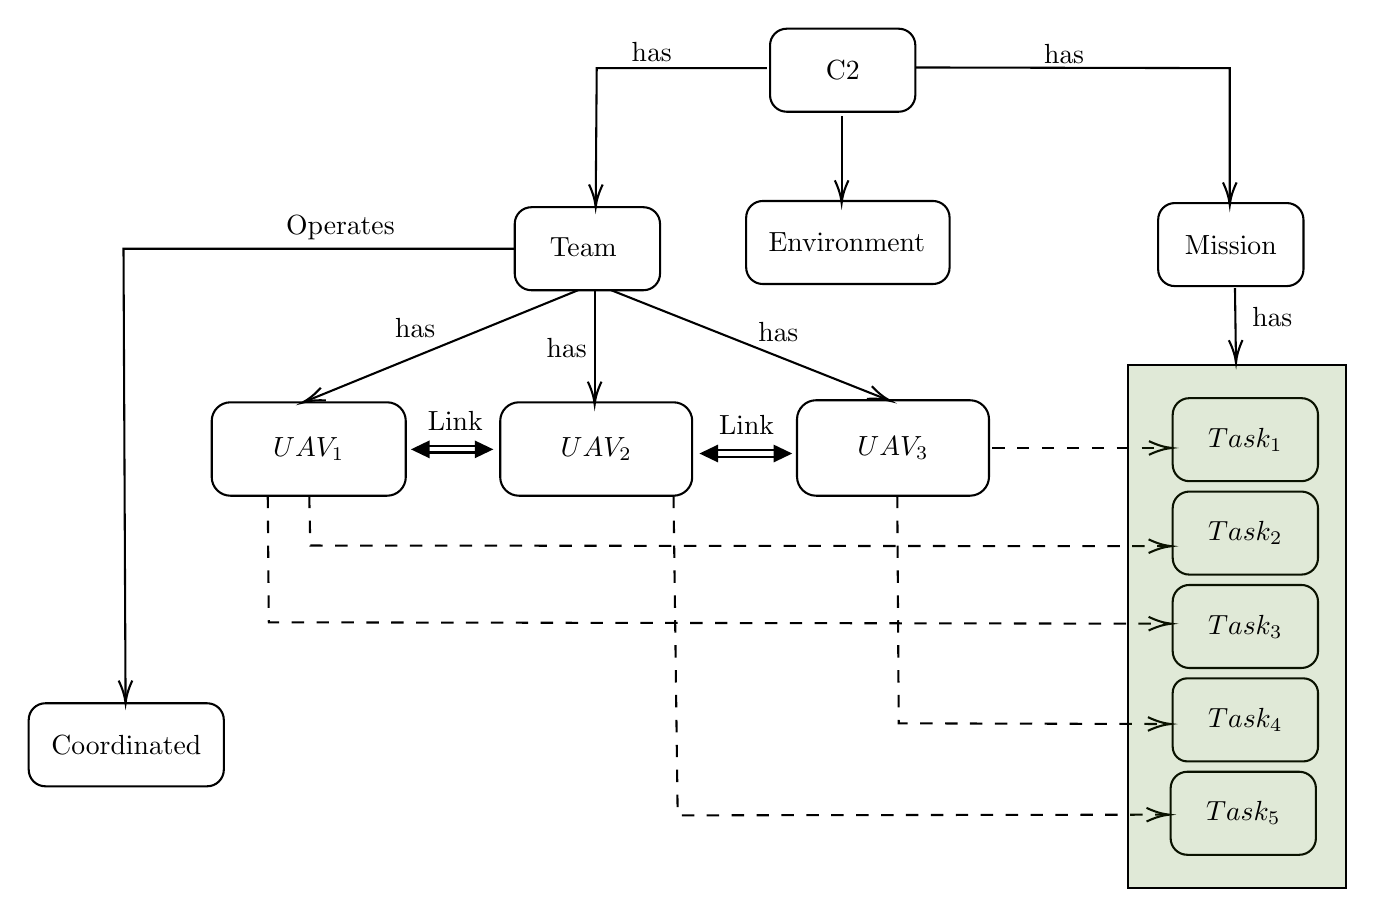
\begin{tikzpicture}[x=0.75pt,y=0.75pt,yscale=-1,xscale=1]
%uncomment if require: \path (0,436); %set diagram left start at 0, and has height of 436

%Flowchart: Alternative Process [id:dp6874708773317039] 
\draw   (557,334) .. controls (557,330.13) and (560.13,327) .. (564,327) -- (620,327) .. controls (623.87,327) and (627,330.13) .. (627,334) -- (627,360) .. controls (627,363.87) and (623.87,367) .. (620,367) -- (564,367) .. controls (560.13,367) and (557,363.87) .. (557,360) -- cycle ;
%Rounded Rect [id:dp02450854228021382] 
\draw   (557,200) .. controls (557,195.58) and (560.58,192) .. (565,192) -- (619,192) .. controls (623.42,192) and (627,195.58) .. (627,200) -- (627,224) .. controls (627,228.42) and (623.42,232) .. (619,232) -- (565,232) .. controls (560.58,232) and (557,228.42) .. (557,224) -- cycle ;
%Rounded Rect [id:dp13119778343107102] 
\draw   (556,380) .. controls (556,375.58) and (559.58,372) .. (564,372) -- (618,372) .. controls (622.42,372) and (626,375.58) .. (626,380) -- (626,404) .. controls (626,408.42) and (622.42,412) .. (618,412) -- (564,412) .. controls (559.58,412) and (556,408.42) .. (556,404) -- cycle ;
%Rounded Rect [id:dp4251383309757243] 
\draw   (557,245) .. controls (557,240.58) and (560.58,237) .. (565,237) -- (619,237) .. controls (623.42,237) and (627,240.58) .. (627,245) -- (627,269) .. controls (627,273.42) and (623.42,277) .. (619,277) -- (565,277) .. controls (560.58,277) and (557,273.42) .. (557,269) -- cycle ;
%Rounded Rect [id:dp16394484975497148] 
\draw   (557,290) .. controls (557,285.58) and (560.58,282) .. (565,282) -- (619,282) .. controls (623.42,282) and (627,285.58) .. (627,290) -- (627,314) .. controls (627,318.42) and (623.42,322) .. (619,322) -- (565,322) .. controls (560.58,322) and (557,318.42) .. (557,314) -- cycle ;
%Rounded Rect [id:dp2393438673799806] 
\draw   (240,108) .. controls (240,103.58) and (243.58,100) .. (248,100) -- (302,100) .. controls (306.42,100) and (310,103.58) .. (310,108) -- (310,132) .. controls (310,136.42) and (306.42,140) .. (302,140) -- (248,140) .. controls (243.58,140) and (240,136.42) .. (240,132) -- cycle ;
%Rounded Rect [id:dp5357554711575779] 
\draw   (94,203) .. controls (94,198.03) and (98.03,194) .. (103,194) -- (178.5,194) .. controls (183.47,194) and (187.5,198.03) .. (187.5,203) -- (187.5,230) .. controls (187.5,234.97) and (183.47,239) .. (178.5,239) -- (103,239) .. controls (98.03,239) and (94,234.97) .. (94,230) -- cycle ;
%Rounded Rect [id:dp49684854051412786] 
\draw   (233,203) .. controls (233,198.03) and (237.03,194) .. (242,194) -- (316.5,194) .. controls (321.47,194) and (325.5,198.03) .. (325.5,203) -- (325.5,230) .. controls (325.5,234.97) and (321.47,239) .. (316.5,239) -- (242,239) .. controls (237.03,239) and (233,234.97) .. (233,230) -- cycle ;
%Rounded Rect [id:dp5565887710836318] 
\draw   (376,202.2) .. controls (376,197.12) and (380.12,193) .. (385.2,193) -- (459.3,193) .. controls (464.38,193) and (468.5,197.12) .. (468.5,202.2) -- (468.5,229.8) .. controls (468.5,234.88) and (464.38,239) .. (459.3,239) -- (385.2,239) .. controls (380.12,239) and (376,234.88) .. (376,229.8) -- cycle ;
%Straight Lines [id:da49767923703046746] 
\draw    (270.5,140) -- (139.52,193.41) ;
\draw [shift={(137.67,194.17)}, rotate = 337.82] [color={rgb, 255:red, 0; green, 0; blue, 0 }  ][line width=0.75]    (10.93,-3.29) .. controls (6.95,-1.4) and (3.31,-0.3) .. (0,0) .. controls (3.31,0.3) and (6.95,1.4) .. (10.93,3.29)   ;

%Straight Lines [id:da655185066924097] 
\draw    (286.5,140) -- (419.14,192.6) ;
\draw [shift={(421,193.33)}, rotate = 201.63] [color={rgb, 255:red, 0; green, 0; blue, 0 }  ][line width=0.75]    (10.93,-3.29) .. controls (6.95,-1.4) and (3.31,-0.3) .. (0,0) .. controls (3.31,0.3) and (6.95,1.4) .. (10.93,3.29)   ;

%Straight Lines [id:da14922683664772962] 
\draw    (278.5,140) -- (278.5,193) ;
\draw [shift={(278.5,195)}, rotate = 270] [color={rgb, 255:red, 0; green, 0; blue, 0 }  ][line width=0.75]    (10.93,-3.29) .. controls (6.95,-1.4) and (3.31,-0.3) .. (0,0) .. controls (3.31,0.3) and (6.95,1.4) .. (10.93,3.29)   ;

%Straight Lines [id:da27148570904007396] 
\draw  [dash pattern={on 4.5pt off 4.5pt}]  (470,216) -- (554.5,216) ;
\draw [shift={(556.5,216)}, rotate = 180] [color={rgb, 255:red, 0; green, 0; blue, 0 }  ][line width=0.75]    (10.93,-3.29) .. controls (6.95,-1.4) and (3.31,-0.3) .. (0,0) .. controls (3.31,0.3) and (6.95,1.4) .. (10.93,3.29)   ;

%Straight Lines [id:da9230667625559809] 
\draw  [dash pattern={on 4.5pt off 4.5pt}]  (424.3,239) -- (425,348.67) -- (554,348.99) ;
\draw [shift={(556,349)}, rotate = 180.15] [color={rgb, 255:red, 0; green, 0; blue, 0 }  ][line width=0.75]    (10.93,-3.29) .. controls (6.95,-1.4) and (3.31,-0.3) .. (0,0) .. controls (3.31,0.3) and (6.95,1.4) .. (10.93,3.29)   ;

%Straight Lines [id:da24437278069710944] 
\draw  [dash pattern={on 4.5pt off 4.5pt}]  (316.5,239) -- (318.5,393) -- (553.33,392.67) ;
\draw [shift={(555.33,392.67)}, rotate = 539.9200000000001] [color={rgb, 255:red, 0; green, 0; blue, 0 }  ][line width=0.75]    (10.93,-3.29) .. controls (6.95,-1.4) and (3.31,-0.3) .. (0,0) .. controls (3.31,0.3) and (6.95,1.4) .. (10.93,3.29)   ;

%Straight Lines [id:da6571794138578118] 
\draw  [dash pattern={on 4.5pt off 4.5pt}]  (141,239) -- (141.5,263) -- (554.33,263.33) ;
\draw [shift={(556.33,263.33)}, rotate = 180.05] [color={rgb, 255:red, 0; green, 0; blue, 0 }  ][line width=0.75]    (10.93,-3.29) .. controls (6.95,-1.4) and (3.31,-0.3) .. (0,0) .. controls (3.31,0.3) and (6.95,1.4) .. (10.93,3.29)   ;

%Straight Lines [id:da5064501468549402] 
\draw  [dash pattern={on 4.5pt off 4.5pt}]  (121,239) -- (121.5,300) -- (554.33,300.66) ;
\draw [shift={(556.33,300.67)}, rotate = 180.09] [color={rgb, 255:red, 0; green, 0; blue, 0 }  ][line width=0.75]    (10.93,-3.29) .. controls (6.95,-1.4) and (3.31,-0.3) .. (0,0) .. controls (3.31,0.3) and (6.95,1.4) .. (10.93,3.29)   ;

%Rounded Rect [id:dp9950378818445779] 
\draw   (363,22) .. controls (363,17.58) and (366.58,14) .. (371,14) -- (425,14) .. controls (429.42,14) and (433,17.58) .. (433,22) -- (433,46) .. controls (433,50.42) and (429.42,54) .. (425,54) -- (371,54) .. controls (366.58,54) and (363,50.42) .. (363,46) -- cycle ;
%Straight Lines [id:da43665394686836234] 
\draw    (279.01,98) -- (279.5,33) -- (361.5,33) ;

\draw [shift={(279,100)}, rotate = 270.43] [color={rgb, 255:red, 0; green, 0; blue, 0 }  ][line width=0.75]    (10.93,-3.29) .. controls (6.95,-1.4) and (3.31,-0.3) .. (0,0) .. controls (3.31,0.3) and (6.95,1.4) .. (10.93,3.29)   ;
%Rounded Rect [id:dp3991546853632061] 
\draw   (550,106) .. controls (550,101.58) and (553.58,98) .. (558,98) -- (612,98) .. controls (616.42,98) and (620,101.58) .. (620,106) -- (620,130) .. controls (620,134.42) and (616.42,138) .. (612,138) -- (558,138) .. controls (553.58,138) and (550,134.42) .. (550,130) -- cycle ;
%Straight Lines [id:da7959398275959729] 
\draw    (433,32.67) -- (584.5,33) -- (584.5,97) ;
\draw [shift={(584.5,99)}, rotate = 270] [color={rgb, 255:red, 0; green, 0; blue, 0 }  ][line width=0.75]    (10.93,-3.29) .. controls (6.95,-1.4) and (3.31,-0.3) .. (0,0) .. controls (3.31,0.3) and (6.95,1.4) .. (10.93,3.29)   ;

%Rounded Rect [id:dp06887225784073736] 
\draw   (351.5,105) .. controls (351.5,100.58) and (355.08,97) .. (359.5,97) -- (441.5,97) .. controls (445.92,97) and (449.5,100.58) .. (449.5,105) -- (449.5,129) .. controls (449.5,133.42) and (445.92,137) .. (441.5,137) -- (359.5,137) .. controls (355.08,137) and (351.5,133.42) .. (351.5,129) -- cycle ;
%Straight Lines [id:da6347850013540862] 
\draw    (397.5,56) -- (397.5,96) ;
\draw [shift={(397.5,98)}, rotate = 270] [color={rgb, 255:red, 0; green, 0; blue, 0 }  ][line width=0.75]    (10.93,-3.29) .. controls (6.95,-1.4) and (3.31,-0.3) .. (0,0) .. controls (3.31,0.3) and (6.95,1.4) .. (10.93,3.29)   ;

%Straight Lines [id:da496152900364659] 
\draw    (587,139) -- (587.47,173) ;
\draw [shift={(587.5,175)}, rotate = 269.2] [color={rgb, 255:red, 0; green, 0; blue, 0 }  ][line width=0.75]    (10.93,-3.29) .. controls (6.95,-1.4) and (3.31,-0.3) .. (0,0) .. controls (3.31,0.3) and (6.95,1.4) .. (10.93,3.29)   ;

%Shape: Rectangle [id:dp01034560128087203] 
\draw  [fill={rgb, 255:red, 65; green, 117; blue, 5 }  ,fill opacity=0.16 ] (535.5,176) -- (640.5,176) -- (640.5,428) -- (535.5,428) -- cycle ;
%Rounded Rect [id:dp6118093658554176] 
\draw   (5.83,347) .. controls (5.83,342.58) and (9.42,339) .. (13.83,339) -- (91.83,339) .. controls (96.25,339) and (99.83,342.58) .. (99.83,347) -- (99.83,371) .. controls (99.83,375.42) and (96.25,379) .. (91.83,379) -- (13.83,379) .. controls (9.42,379) and (5.83,375.42) .. (5.83,371) -- cycle ;
%Straight Lines [id:da29333902336318574] 
\draw    (240,120) -- (51.5,120) -- (52.49,337) ;
\draw [shift={(52.5,339)}, rotate = 269.74] [color={rgb, 255:red, 0; green, 0; blue, 0 }  ][line width=0.75]    (10.93,-3.29) .. controls (6.95,-1.4) and (3.31,-0.3) .. (0,0) .. controls (3.31,0.3) and (6.95,1.4) .. (10.93,3.29)   ;

%Straight Lines [id:da010804313456069026] 
\draw    (198,215.17) -- (221.67,215.17)(198,218.17) -- (221.67,218.17) ;
\draw [shift={(229.67,216.67)}, rotate = 180] [fill={rgb, 255:red, 0; green, 0; blue, 0 }  ][line width=0.75]  [draw opacity=0] (8.93,-4.29) -- (0,0) -- (8.93,4.29) -- cycle    ;
\draw [shift={(190,216.67)}, rotate = 0] [fill={rgb, 255:red, 0; green, 0; blue, 0 }  ][line width=0.75]  [draw opacity=0] (8.93,-4.29) -- (0,0) -- (8.93,4.29) -- cycle    ;
%Straight Lines [id:da46176583183237185] 
\draw    (337,217.17) -- (365.67,217.17)(337,220.17) -- (365.67,220.17) ;
\draw [shift={(373.67,218.67)}, rotate = 180] [fill={rgb, 255:red, 0; green, 0; blue, 0 }  ][line width=0.75]  [draw opacity=0] (8.93,-4.29) -- (0,0) -- (8.93,4.29) -- cycle    ;
\draw [shift={(329,218.67)}, rotate = 0] [fill={rgb, 255:red, 0; green, 0; blue, 0 }  ][line width=0.75]  [draw opacity=0] (8.93,-4.29) -- (0,0) -- (8.93,4.29) -- cycle    ;

% Text Node
\draw (273,119) node  [align=left] {Team};
% Text Node
\draw (592,212) node   {$Task_{1}$};
% Text Node
\draw (592,257) node   {$Task_{2}$};
% Text Node
\draw (592,302) node   {$Task_{3}$};
% Text Node
\draw (592,347) node   {$Task_{4}$};
% Text Node
\draw (591,392) node   {$Task_{5}$};
% Text Node
\draw (140.75,216.5) node   {$UAV_{1}$};
% Text Node
\draw (279.25,216.5) node   {$UAV_{2}$};
% Text Node
\draw (422.25,216) node   {$UAV_{3}$};
% Text Node
\draw (367,160) node  [align=left] {has};
% Text Node
\draw (265,168) node  [align=left] {has};
% Text Node
\draw (192,158.33) node  [align=left] {has};
% Text Node
\draw (398,34) node  [align=left] {C2};
% Text Node
\draw (306,25) node  [align=left] {has};
% Text Node
\draw (585,118) node  [align=left] {Mission};
% Text Node
\draw (400,117) node  [align=left] {Environment};
% Text Node
\draw (504.67,26) node  [align=left] {has};
% Text Node
\draw (605,153) node  [align=left] {has};
% Text Node
\draw (52.83,359) node  [align=left] {Coordinated};
% Text Node
\draw (156,110) node  [align=left] {Operates};
% Text Node
\draw (351.67,205) node  [align=left] {Link};
% Text Node
\draw (211.33,203) node  [align=left] {Link};


\end{tikzpicture}}
\label{example1}
\caption{A C2 system instance representing the tasks allocation presented in \cite{Schwarzrock2017}}
\end{figure}

In general, we abstract the representation where the MDSPL of a C2 System comprises a mission, an environment, a set of entities, and resourcess available to perform the mission. Figure \ref{meta01} shows the meta-model representing this structural view of the MDSPL of the C2 System.  The entities that perform the allocated tasks can be grouped in teams and this entity operates on a specific C2 Approach chosen according to the mission and requirements. The awareness sharing between the members occurs through links of communication defined by the C2 Approach selected. In terms of this proposal, resources are represented within members' onboard features.

To provide C2 Agility to this model, the MDSPL must first be able to identify changes in circumstances. Indeed, members' onboard sensors  sense new environment conditions. Members are also aware of their status, e.g., battery level. Moreover, at the global level, there is a list of tasks ($T$) to be performed that characterize the mission. Changes in this list represents mission modification. By leveraging the reconfiguration capability of each member DSPL as well as their coordination capability, eventually performing task allocation and/or changing the C2 Approach, in all cases guided by QoS constraints, the MDSPL of the C2 System enjoys agility. 

An assumption of our model is that there is no member collaboration within a single task, i.e., we have only one member per task but we can have more than one tasks allocated to a member. Still, there is an interaction between the members, with awareness sharing according to the C2 Approach that is being operated. This interaction contributes with the configuration adopted by the member because the members  configuring themselves to best perform allocated tasks. Furthermore, environment changes such as risk level increase or security aspects that require an external observation and action are outside the scope of this work.

\begin{center}
    \figura[!h]{Meta-Model-Static}{Meta-model representing structure of the MDSPL of the  C2 System}{meta01}{width=1\textwidth}
\end{center}

%due to the exponential complexity inserted into the model, becoming it unfeasible.

\subsubsection{Fine-grained Structure: Feature Model}

As previously explained, in the C2 System, the team comprises members that execute the tasks allocated to each of them. Each member $e$ belongs to a team that is defined as a set $E=\{e_1, e_2, ..., e_n\}$ of members. These elements are modelled as a DSPL and thereby they have control mechanisms to monitor context changes and adapt themselves to be able to perform tasks in new circumstances. This adaptation capability provides C2 Approach Agility.

The DSPL of a member $e_k \in E$ is statically described by an attributed-based feature model (FM) to identify member variability, whereby
%and the notation is $ \llbracket e_k \rrbracket_{FM}$. To simplify the representation, 
 $ \llbracket e_k \rrbracket$ denotes the set of valid configurations from the FM of member $e_k$. The features in FM model both the environment (features represent sensors and their value as attributes)  and the self (functional status and some internal characteristic, e.g. battery level) of each C2 System member. Further, the DSPLs are goal-oriented~\cite{BencomoHA12}, that is, they aim at satisfying goals and reconfiguring for that purpose, if necessary. The goals of each DSPL are a partial view on the mission of the C2 System (its sets of tasks). Such  view is computed at runtime via task allocation (described in Section~\ref{sec:behavior}).  Initially, we consider functional goals, but we expect to handle cost and other attributes as the proposal is refined.  


\subsection{Roles and Responsibilities} \label{sec:rolesResponsibilities}
 
Motivated by the idea of multiple feedback loops to monitor multiple concerns presented by \textit{Vogel et al.}~\cite{Vogel01}, our proposal brings a similar concept presented in a different way. As proposed by \textit{Arcaini et. al.}~\cite{MAPE01}, each layer presented by the Figure \ref{mape01} can be represented by a role or responsibility of the system. This concept is compatible with the C2 application domain and it is called \textit{roles or responsibilities separation} \cite{Alberts2000}. In the C2 Domain, it is essential to define the members roles because their execution are guided by the responsibilities related to these roles. Indeed, roles defines the members' behaviour.

Table \ref{table:table04} lists the three roles and corresponding responsibilities identified in domain. They are orthogonal to the component's view shown in Figure \ref{mape01}. Assuming that each member is modeled as a specific component, at any point in time, the same member can be playing more than one role. Conversely, each role can be played by different members. Further, a member can assume one or more roles during system execution, and these roles performed can be assumed simultaneously or sequentially in runtime. Therefore, each role can be represented as a dynamic view on the layered component's architecture.

% TODO: it would improve presentation here if we provided a 1-paragraph example of role-to-member mapping here relating to the concrete example of figure example1, which we use in the Structural Specification subsection.
%%%%%% OK %%%%%%%%%%

\begin{table}[ht]
	\small
	\fontsize{10}{10}\selectfont
	\centering
	\caption{C2 System roles and responsibilities}
	\label{table:table04}
	
	\begin{tabular}{ccc}
	\hline
		\textbf{Role}
		& \textbf{Abbrev.}
		& \textbf{Responsibility} \\ [1ex]
	\hline	
	
	Executor & EX & Perform mission tasks  \\[1ex]
	Task Allocator & TA & Allocate the tasks among executors \\[1ex]
	C2 Approach Selector & C2A & Select an appropriate C2 Approach based on the resources \\[1ex]
	\hline
	\end{tabular}
\end{table} 

Based on the example showed in Figure \ref{example1}, let's define some example roles to the members as following:

\hspace{4cm} $UAV_1 \mapsto \{Executor\}$

\hspace{4cm} $UAV_2 \mapsto \{Task Allocator, C2 Approach Selector\}$

\hspace{4cm} $UAV_3 \mapsto \{Executor\}$

The Executors run a virtual MAPE-K loop, i.e., lowest loop in Figure \ref{mape01}, to monitor and act according to circumstance changes. In a similar way, the $UAV_2$ has the ability to allocate tasks and to select the C2 Approach to be used by the team.

Ultimately, roles deals with context changes, i.e., changes in the mission, the environment, or in the self. The response given by each role  when circumstance changes defines the system adaptation process, and the possibilities are the following:

\begin{enumerate}
    \item All executors in the team  are performing the tasks with no special adjustments in runtime. This is the normal situation;
    \item Context changes cause a reconfiguration in one or more executors. This represents C2 Approach Agility, which indicates the capability of the system to adapt itself with no C2 Approach change. In this case, with information about the tasks to be performed, some executors will reconfigure themselves to try to stabilize the system. The Task Allocator may also try to reallocate all possible tasks available to complete the configuration step if necessary;
    \item In case C2 Approach Agility does not work, it is necessary to try a C2 Approach change to deal with the new circumstance. The C2 Approach Selector will define the new C2 strategy, and the executors will be organized according to a C2 Approach selected and will analyze if the tasks can be performed. The new coordination may impact the task allocation procedure, so the Task Allocator may be called to redistribute tasks satisfying some QAs among the executors. The capability of finding and transitioning to a C2 Approach to deal with context changes defines the C2 Maneuver Agility level;
    \item No executors configuration nor C2 Approach are suitable to perform the tasks after changes in circumstances. Unfeasible tasks are recorded and the C2 System proceeds with any subsequent tasks.
\end{enumerate}


\subsection{Behavioral Specification} \label{sec:behavior}

A C2 System applies a set of members to perform a mission and they need to be able to adapt themselves according to circumstance changes. The members can operate in this dynamic scenario due to the awareness and context information exchange. Addressing the dynamic behavior requires a communication mechanism to guarantee an information exchange between the processes that are parts of C2 Agility. Members are thus stateful entities that interact in prescribed ways.  To precisely model this scenario, we rely on formal grounds, whereby we leverage a Channel System (CS) to describe the behavior of the C2 System, which we detail next. 

According to Section~\ref{sec:rolesResponsibilities}, the C2 System is represented by three roles: C2 Approach Selector (C2A), Task Allocator (TA), and Executor (EX). We map instances of each role to one or more PGs in the corresponding CS. This structure is able to represent the communication among the these three roles, i.e., PGs, working in a parallel way.

Equation \eqref{pg01} shows the Channel System ($CS_{UAV}$) of the C2 System, with instances of these three roles as PGs running in a parallel way, that represents the example of Figure \ref{example1} with the roles assignment made as example in the same Section previously cited.

\begin{equation}
\label{pg01}
    CS_{UAV} = [C2A | TA | EX_1 | EX_2]
\end{equation}

A static view of Equation~\eqref{pg01}, with its channels, can be seen in Figure~\ref{pg}. Each member with index $k$ has a private asynchronous channel $m_k$ that is used by the task allocator to dispatch tasks to be performed. The channels $b_k$ are used by the member $k$ to send tasks not suitable to be performed for a new allocation. The channel $b_2$ is used to scale the tasks issues to the C2 Approach selector to identify another C2 Approach suitable to the entities perform the tasks.  Additionally, $CS_{UAV}$ corresponds to the C2 System whose coarse-grained structure is represented in Figure~\ref{example1}, assuming that, at a given point in time, the following role-to-member mapping holds: 

\begin{center}
\begin{equation}
\{ C2A \mapsto \{UAV_2\}  , TA \mapsto \{UAV_2\} ,  EX \mapsto \{UAV_1, UAV_3\}\}
 \end{equation}
\end{center}


\begin{figure}[h]
\centering



\tikzset{every picture/.style={line width=0.75pt}} %set default line width to 0.75pt        

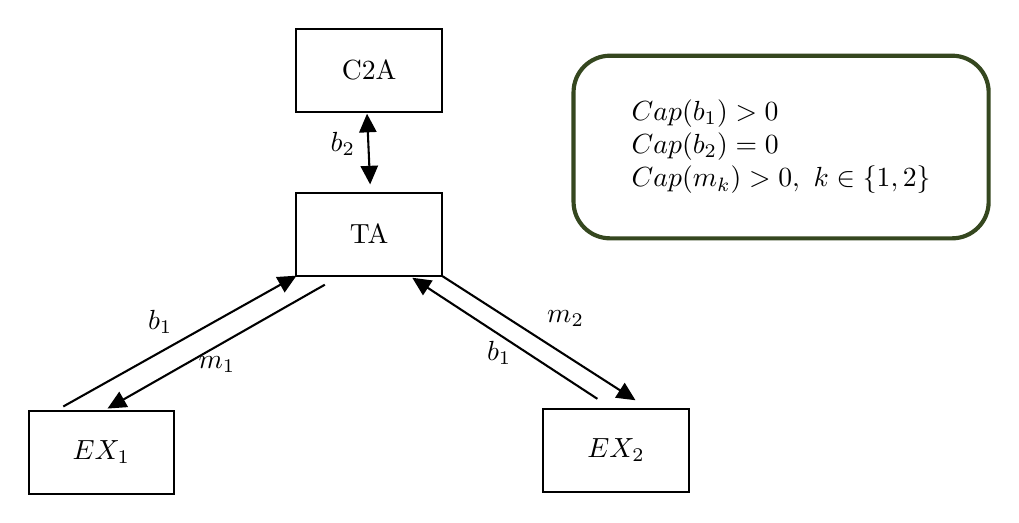
\begin{tikzpicture}[x=0.75pt,y=0.75pt,yscale=-1,xscale=1]
%uncomment if require: \path (0,268); %set diagram left start at 0, and has height of 268

%Shape: Rectangle [id:dp7793135649662085] 
\draw   (158,110) -- (228,110) -- (228,150) -- (158,150) -- cycle ;
%Shape: Rectangle [id:dp8388066725390221] 
\draw   (158,31) -- (228,31) -- (228,71) -- (158,71) -- cycle ;
%Shape: Rectangle [id:dp48691256180587716] 
\draw   (277,214) -- (347,214) -- (347,254) -- (277,254) -- cycle ;
%Shape: Rectangle [id:dp8836932328283702] 
\draw   (29,215) -- (99,215) -- (99,255) -- (29,255) -- cycle ;
%Straight Lines [id:da3337977868298102] 
\draw    (192.09,74) -- (193.41,104) ;
\draw [shift={(193.5,106)}, rotate = 267.47] [fill={rgb, 255:red, 0; green, 0; blue, 0 }  ][line width=0.75]  [draw opacity=0] (8.93,-4.29) -- (0,0) -- (8.93,4.29) -- cycle    ;
\draw [shift={(192,72)}, rotate = 87.47] [fill={rgb, 255:red, 0; green, 0; blue, 0 }  ][line width=0.75]  [draw opacity=0] (8.93,-4.29) -- (0,0) -- (8.93,4.29) -- cycle    ;
%Straight Lines [id:da7136052167478543] 
\draw    (171.67,154.33) -- (68.74,213.01) ;
\draw [shift={(67,214)}, rotate = 330.31] [fill={rgb, 255:red, 0; green, 0; blue, 0 }  ][line width=0.75]  [draw opacity=0] (8.93,-4.29) -- (0,0) -- (8.93,4.29) -- cycle    ;

%Straight Lines [id:da5349782032446363] 
\draw    (228,150) -- (319.65,208.92) ;
\draw [shift={(321.33,210)}, rotate = 212.74] [fill={rgb, 255:red, 0; green, 0; blue, 0 }  ][line width=0.75]  [draw opacity=0] (8.93,-4.29) -- (0,0) -- (8.93,4.29) -- cycle    ;

%Straight Lines [id:da1199439366931846] 
\draw    (45.67,213) -- (156.26,150.98) ;
\draw [shift={(158,150)}, rotate = 510.71] [fill={rgb, 255:red, 0; green, 0; blue, 0 }  ][line width=0.75]  [draw opacity=0] (8.93,-4.29) -- (0,0) -- (8.93,4.29) -- cycle    ;

%Straight Lines [id:da14294220152856596] 
\draw    (303,209.33) -- (215.51,152.09) ;
\draw [shift={(213.83,151)}, rotate = 393.19] [fill={rgb, 255:red, 0; green, 0; blue, 0 }  ][line width=0.75]  [draw opacity=0] (8.93,-4.29) -- (0,0) -- (8.93,4.29) -- cycle    ;

%Rounded Rect [id:dp3574279176331121] 
\draw  [color={rgb, 255:red, 53; green, 71; blue, 31 }  ,draw opacity=1 ][line width=1.5]  (291.5,61.6) .. controls (291.5,51.88) and (299.38,44) .. (309.1,44) -- (473.9,44) .. controls (483.62,44) and (491.5,51.88) .. (491.5,61.6) -- (491.5,114.4) .. controls (491.5,124.12) and (483.62,132) .. (473.9,132) -- (309.1,132) .. controls (299.38,132) and (291.5,124.12) .. (291.5,114.4) -- cycle ;

% Text Node
\draw (193,51) node  [align=left] {C2A};
% Text Node
\draw (193,130) node  [align=left] {TA};
% Text Node
\draw (64,235) node   {$EX_{1}$};
% Text Node
\draw (312,234) node   {$EX_{2}$};
% Text Node
\draw (92.33,172.33) node   {$b_{1}$};
% Text Node
\draw (255.67,187.33) node   {$b_{1}$};
% Text Node
\draw (119.67,193) node   {$m_{1}$};
% Text Node
\draw (287.67,170.67) node   {$m_{2}$};
% Text Node
\draw (180.33,86.33) node   {$b_{2}$};
% Text Node
\draw (391.5,88) node   {$ \begin{array}{l}
Cap( b_{1})  >0\\
Cap( b_{2}) =0\\
Cap( m_{k})  >0,\ k\in \{1,2\}
\end{array}$};


\end{tikzpicture}
\label{pg}
\caption{PG static view with \textit{n} entities as executors}
\end{figure}

% REMOVED, FOR WHILE, BY THE ADVISOR.
%To simplify, we will use the notation $\{EX\}|_{1}^n$ to represent the set of executors' program graphs $[EX_1 | EX_2 | ... | EX_n]$, where $n = |E|$ and the list of members $E$ is received by the channel system as a parameter. With this, the equation \eqref{pg01} can be rewritten as following.

%\begin{equation}
%\label{pg02}
%    CS_{S} = [C2A | TA | \{EX\}_{1}^n]
%\end{equation}

%A proposal to model this communication process among the parallel program graphs is using a buffer structure as a first-in-first-out queue, when the communications are asynchronous, or a handshake mechanism when a synchronize is required. These communication structures are called channels \cite{baier}. 


More generally, we leverage \textit{parameterized Chanel System} to abstract over specific instances of the PGs representing roles. Accordingly, some variables in these PGs are turned into parameters. Specifically, let $ap$ be a C2 Approach selected in $\Omega = \{Edge, De-Conflicted, Coord, Conflicted, Collab\}$, $T_0$ a set of tasks, $M$ the of all set of tasks $t$ that can be allocated,  and $E = \{e_1, e_2, ..., e_n\}$ a set of executors' FMs. Equation \ref{pg03} shows the  parameterized CS with the type definition for each parameter. 

\begin{equation}
\label{pg03}
\begin{split}
CS_S(ap:\omega, T_0: &\powerset(M), E:\{FM_1, FM_2, ..., FM_n\})=\\
&=[ C2A(ap) | TA(T_0) | EX(e_1) | EX(e_2) | ... | EX(e_k) ]
\end{split}
\end{equation}

The intended semantics is as follows. $ap$ is a C2 Approach to be used in the beginning and $T_0$ is a initial set of tasks $\{t_1, t_2, ..., t_k\}$ representing the current mission, and $E$ is the set of executors ${e_1, e_2, ..., e_n}$. To satisfy $g_0$, it is mandatory to have $(ap \in \Omega)$ and $(T_0 \subseteq M)$. For each executor $e_j$,  an instance $EX$ of PG is created. All such instances are composed like in a plain CS. In the following, we detail the abstracted PGs.


%\begin{equation}
%\label{pg02}
%    CS_{S} = CS_S(ap:\omega, T_0:M, E:\{FM_1, FM_2, ..., FM_n\})
%\end{equation}

%From the above equation, we can provide specific arguments $(ap, T_0, E)$ with $E=\{e_1, e_2, ..., e_k\}$ to create a CS formed by specific instances of PG based on these arguments, which will be used to validate the initial guard of each PG. 

\subsubsection{C2 Approach Selector}

The PG of C2 Approach Selector ($PG_{C2A}$) is shown in Figure \ref{c2a}. It represents the C2 Approach (C2A) selection role with its elements and definitions. The element \textit{e}, i.e., the executor, which belongs to the set $E$, is represented by its FM and it has a valid  configuration $c$ such that  $c \in \llbracket e \rrbracket $.

%\begin{center}
%\begin{equation}
%c \in \llbracket e \rrbracket 
%\end{equation}
%\end{center}

%and this configuration represents one state of $e$ within the set of all possible valid configurations that can be employed during a given mission $T_i$ execution according to circumstance changes.

\begin{figure}[h]
\centering



\tikzset{every picture/.style={line width=0.75pt}} %set default line width to 0.75pt        

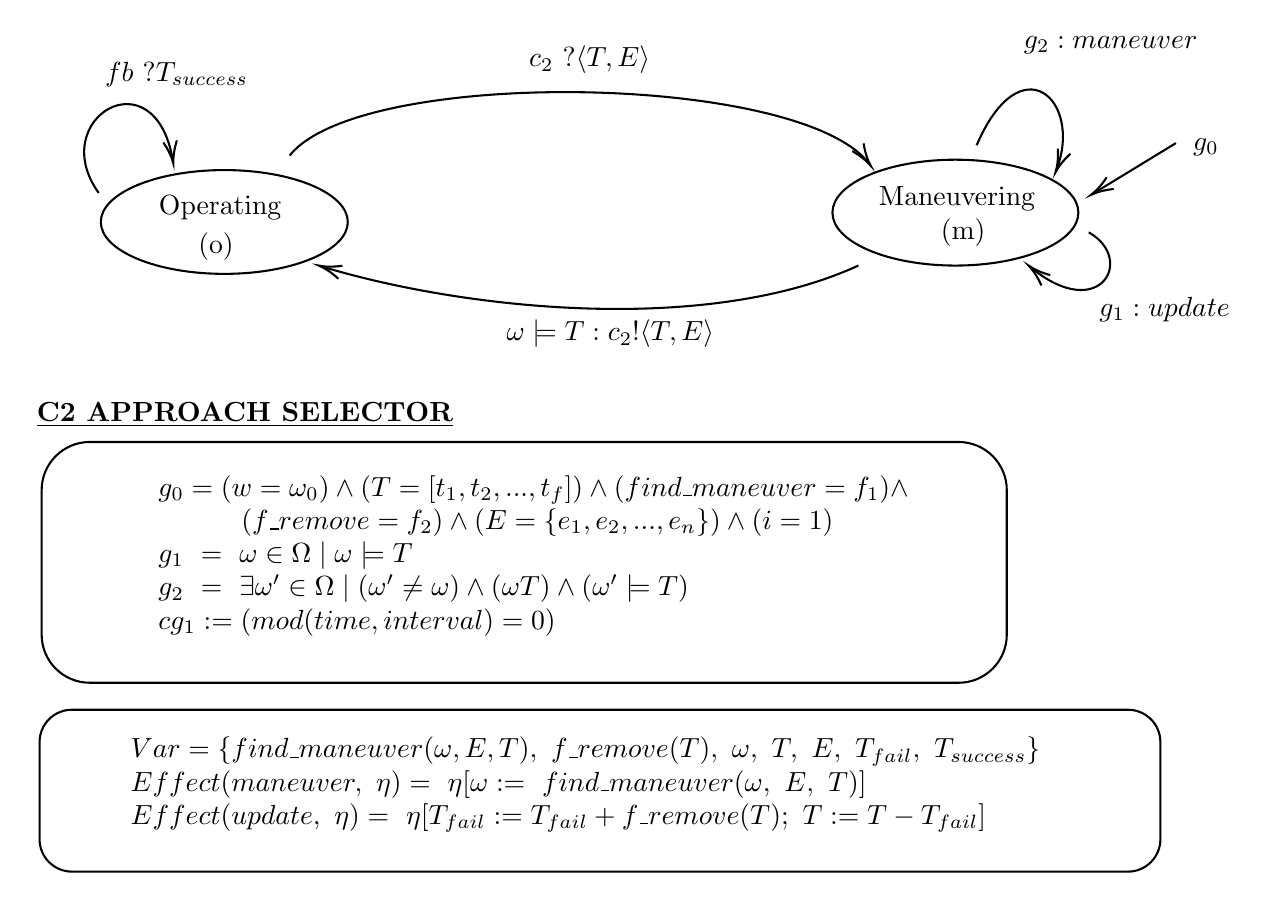
\begin{tikzpicture}[x=0.75pt,y=0.75pt,yscale=-1,xscale=1]
%uncomment if require: \path (0,420); %set diagram left start at 0, and has height of 420

%Curve Lines [id:da9480858267519683] 
\draw    (135.5,66) .. controls (169.16,23.43) and (380.22,25.94) .. (414.52,69.66) ;
\draw [shift={(415.5,71)}, rotate = 235.44] [color={rgb, 255:red, 0; green, 0; blue, 0 }  ][line width=0.75]    (10.93,-3.29) .. controls (6.95,-1.4) and (3.31,-0.3) .. (0,0) .. controls (3.31,0.3) and (6.95,1.4) .. (10.93,3.29)   ;
%Shape: Ellipse [id:dp6594609066072359] 
\draw   (44.5,98) .. controls (44.5,84.19) and (71.14,73) .. (104,73) .. controls (136.86,73) and (163.5,84.19) .. (163.5,98) .. controls (163.5,111.81) and (136.86,123) .. (104,123) .. controls (71.14,123) and (44.5,111.81) .. (44.5,98) -- cycle ;
%Shape: Ellipse [id:dp873836537729809] 
\draw   (397,93.5) .. controls (397,79.42) and (423.53,68) .. (456.25,68) .. controls (488.97,68) and (515.5,79.42) .. (515.5,93.5) .. controls (515.5,107.58) and (488.97,119) .. (456.25,119) .. controls (423.53,119) and (397,107.58) .. (397,93.5) -- cycle ;
%Curve Lines [id:da21020703050779688] 
\draw    (466.5,61) .. controls (487.68,11.75) and (517.59,39.15) .. (505.1,72.47) ;
\draw [shift={(504.5,74)}, rotate = 292.38] [color={rgb, 255:red, 0; green, 0; blue, 0 }  ][line width=0.75]    (10.93,-3.29) .. controls (6.95,-1.4) and (3.31,-0.3) .. (0,0) .. controls (3.31,0.3) and (6.95,1.4) .. (10.93,3.29)   ;
%Curve Lines [id:da14662580418826565] 
\draw    (520.5,103) .. controls (543.16,115.81) and (526.03,147.04) .. (493.02,120.26) ;
\draw [shift={(491.5,119)}, rotate = 400.46000000000004] [color={rgb, 255:red, 0; green, 0; blue, 0 }  ][line width=0.75]    (10.93,-3.29) .. controls (6.95,-1.4) and (3.31,-0.3) .. (0,0) .. controls (3.31,0.3) and (6.95,1.4) .. (10.93,3.29)   ;
%Straight Lines [id:da37650774099478246] 
\draw    (562.5,60) -- (523.21,83.96) ;
\draw [shift={(521.5,85)}, rotate = 328.63] [color={rgb, 255:red, 0; green, 0; blue, 0 }  ][line width=0.75]    (10.93,-3.29) .. controls (6.95,-1.4) and (3.31,-0.3) .. (0,0) .. controls (3.31,0.3) and (6.95,1.4) .. (10.93,3.29)   ;
%Rounded Rect [id:dp20897962983691354] 
\draw   (16,227.2) .. controls (16,214.39) and (26.39,204) .. (39.2,204) -- (457.8,204) .. controls (470.61,204) and (481,214.39) .. (481,227.2) -- (481,296.8) .. controls (481,309.61) and (470.61,320) .. (457.8,320) -- (39.2,320) .. controls (26.39,320) and (16,309.61) .. (16,296.8) -- cycle ;
%Rounded Rect [id:dp6489541210438411] 
\draw   (15,348.6) .. controls (15,339.98) and (21.98,333) .. (30.6,333) -- (539.4,333) .. controls (548.02,333) and (555,339.98) .. (555,348.6) -- (555,395.4) .. controls (555,404.02) and (548.02,411) .. (539.4,411) -- (30.6,411) .. controls (21.98,411) and (15,404.02) .. (15,395.4) -- cycle ;
%Curve Lines [id:da07722007259294938] 
\draw    (43.5,84) .. controls (17.76,48.36) and (70.43,16.64) .. (79.25,68.41) ;
\draw [shift={(79.5,70)}, rotate = 261.57] [color={rgb, 255:red, 0; green, 0; blue, 0 }  ][line width=0.75]    (10.93,-3.29) .. controls (6.95,-1.4) and (3.31,-0.3) .. (0,0) .. controls (3.31,0.3) and (6.95,1.4) .. (10.93,3.29)   ;
%Curve Lines [id:da13961356622291943] 
\draw    (409.5,119) .. controls (335.87,152.83) and (218.68,140.13) .. (150.52,119.31) ;
\draw [shift={(149.5,119)}, rotate = 377.15999999999997] [color={rgb, 255:red, 0; green, 0; blue, 0 }  ][line width=0.75]    (10.93,-3.29) .. controls (6.95,-1.4) and (3.31,-0.3) .. (0,0) .. controls (3.31,0.3) and (6.95,1.4) .. (10.93,3.29)   ;

% Text Node
\draw (102,91) node   [align=left] {Operating};
% Text Node
\draw (457,87) node   [align=left] {Maneuvering};
% Text Node
\draw (280,20) node    {$c_{2} \ ?\langle T,E\rangle $};
% Text Node
\draw (577,62) node    {$g_{0}$};
% Text Node
\draw (557,140) node    {$g_{1} :update$};
% Text Node
\draw (531,13) node    {$g_{2} :maneuver$};
% Text Node
\draw (253,259) node    {$ \begin{array}{l}
g_{0} =( w=\omega _{0}) \land ( T=[ t_{1} ,t_{2} ,...,t_{f}]) \land ( find\_maneuver=f_{1}) \land \\
\ \ \ \ \ \ \ \ \ ( f\_remove=f_{2}) \land ( E=\{e_{1} ,e_{2} ,...,e_{n}\}) \land ( i=1)\\
g_{1} \ =\ \nexists \omega \in \Omega \mid \omega \models T\\
g_{2} \ =\ \exists \omega '\in \Omega \mid ( \omega '\neq \omega ) \land ( \omega \nvDash T) \land ( \omega '\models T)\\
cg_{1} :=( mod( time,interval) =0)
\end{array}$};
% Text Node
\draw (460,103) node   [align=left] {(m)};
% Text Node
\draw (100,110) node   [align=left] {(o)};
% Text Node
\draw (278,369) node    {$ \begin{array}{l}
Var=\{find\_maneuver( \omega ,E,T) ,\ f\_remove( T) ,\ \omega ,\ T,\ E,\ T_{fail} ,\ T_{success}\}\\
Effect( maneuver,\ \eta ) =\ \eta [ \omega :=\ find\_maneuver( \omega ,\ E,\ T)]\\
Effect( update,\ \eta ) =\ \eta [ T_{fail} :=T_{fail} +f\_remove( T) ;\ T:=T-T_{fail}]
\end{array}$};
% Text Node
\draw (81,27) node    {$fb\ ?T_{success}$};
% Text Node
\draw (114,191) node   [align=left] {\textbf{\underline{C2 APPROACH SELECTOR}}};
% Text Node
\draw (290,152) node    {$\omega \models T:c_{2} !\langle T,E\rangle $};


\end{tikzpicture}
\label{c2a}
\caption{C2 Approach selector PG}
\end{figure}

 $PG_{C2A}$ uses functions $f\_remove$ and $find\_maneuver$ to encapsulate operations over variables:
\begin{itemize}
    \item $f\_remove$:  generates a new set of tasks $T' \subseteq T$ such that $\omega \models T'$;
    \item $find\_maneuver$: searches for another C2 Approach ($\omega$) that is capable to execute all set of tasks $T$, so called $\omega \models T$;
\end{itemize}

Essentially, the C2 Approach selector receives a team of members, a set of tasks as a mission, and an initial C2 approach to be operated by the members during the tasks execution. Thereby, it analyses if the C2 Approach defined is suitable to the mission and, if not, it tries to maneuver to another C2 Approach and write the selection in the buffer to the next level, and tries to reallocate them among the members according to quality attributes. 

\subsubsection{Task Allocator} 

The PG responsible for the task allocation is shown in Figure \ref{ta}, so-called PG Task Allocator ($PG_{TA}$). It works on a list of tasks $T$ and members $E$ and finds an allocation applying the functions \textit{f\_alloc} and \textit{alloc}. This last one returns a list of pairs $[\langle k,T'_k \rangle]$ where $k$ is the index of the member $e_k \in E$, with the tasks $T'_k \subseteq T$ allocated. This list is feed by the function \textit{f\_alloc} that performs the allocation algorithm. In case of problems to allocate tasks, TA calls C2A to change C2 Approach and tries to perform a new allocation.

\begin{figure}
\centering



\tikzset{every picture/.style={line width=0.75pt}} %set default line width to 0.75pt        

\begin{tikzpicture}[x=0.75pt,y=0.75pt,yscale=-1,xscale=1]
%uncomment if require: \path (0,726); %set diagram left start at 0, and has height of 726

%Curve Lines [id:da9480858267519683] 
\draw    (230.5,181) .. controls (264.16,138.43) and (373.78,135.06) .. (406.05,178.66) ;
\draw [shift={(407,180)}, rotate = 235.44] [color={rgb, 255:red, 0; green, 0; blue, 0 }  ][line width=0.75]    (10.93,-3.29) .. controls (6.95,-1.4) and (3.31,-0.3) .. (0,0) .. controls (3.31,0.3) and (6.95,1.4) .. (10.93,3.29)   ;
%Shape: Ellipse [id:dp6594609066072359] 
\draw   (120.5,208) .. controls (120.5,194.19) and (147.14,183) .. (180,183) .. controls (212.86,183) and (239.5,194.19) .. (239.5,208) .. controls (239.5,221.81) and (212.86,233) .. (180,233) .. controls (147.14,233) and (120.5,221.81) .. (120.5,208) -- cycle ;
%Shape: Ellipse [id:dp873836537729809] 
\draw   (397,201.5) .. controls (397,187.42) and (423.53,176) .. (456.25,176) .. controls (488.97,176) and (515.5,187.42) .. (515.5,201.5) .. controls (515.5,215.58) and (488.97,227) .. (456.25,227) .. controls (423.53,227) and (397,215.58) .. (397,201.5) -- cycle ;
%Curve Lines [id:da14662580418826565] 
\draw    (514.5,424) .. controls (567.96,419.05) and (594.96,385.68) .. (603.25,341.35) ;
\draw [shift={(603.5,340)}, rotate = 460.08] [color={rgb, 255:red, 0; green, 0; blue, 0 }  ][line width=0.75]    (10.93,-3.29) .. controls (6.95,-1.4) and (3.31,-0.3) .. (0,0) .. controls (3.31,0.3) and (6.95,1.4) .. (10.93,3.29)   ;
%Straight Lines [id:da37650774099478246] 
\draw    (232.5,14) -- (263.11,24.36) ;
\draw [shift={(265,25)}, rotate = 198.7] [color={rgb, 255:red, 0; green, 0; blue, 0 }  ][line width=0.75]    (10.93,-3.29) .. controls (6.95,-1.4) and (3.31,-0.3) .. (0,0) .. controls (3.31,0.3) and (6.95,1.4) .. (10.93,3.29)   ;
%Shape: Ellipse [id:dp8139093405894636] 
\draw   (121,419) .. controls (121,405.19) and (147.53,394) .. (180.25,394) .. controls (212.97,394) and (239.5,405.19) .. (239.5,419) .. controls (239.5,432.81) and (212.97,444) .. (180.25,444) .. controls (147.53,444) and (121,432.81) .. (121,419) -- cycle ;
%Shape: Ellipse [id:dp08678607998247811] 
\draw   (391,418) .. controls (391,404.19) and (417.53,393) .. (450.25,393) .. controls (482.97,393) and (509.5,404.19) .. (509.5,418) .. controls (509.5,431.81) and (482.97,443) .. (450.25,443) .. controls (417.53,443) and (391,431.81) .. (391,418) -- cycle ;
%Shape: Ellipse [id:dp07482494496489733] 
\draw   (270,28) .. controls (270,14.75) and (296.53,4) .. (329.25,4) .. controls (361.97,4) and (388.5,14.75) .. (388.5,28) .. controls (388.5,41.25) and (361.97,52) .. (329.25,52) .. controls (296.53,52) and (270,41.25) .. (270,28) -- cycle ;
%Curve Lines [id:da6759956440889884] 
\draw    (123.5,226) .. controls (100.84,271.31) and (108.27,364.16) .. (126.65,401.34) ;
\draw [shift={(127.5,403)}, rotate = 242.18] [color={rgb, 255:red, 0; green, 0; blue, 0 }  ][line width=0.75]    (10.93,-3.29) .. controls (6.95,-1.4) and (3.31,-0.3) .. (0,0) .. controls (3.31,0.3) and (6.95,1.4) .. (10.93,3.29)   ;
%Curve Lines [id:da9572857730465772] 
\draw    (234.22,228.76) .. controls (260.49,268.16) and (260.11,371.42) .. (234.5,399) ;
\draw [shift={(233,227)}, rotate = 54.11] [color={rgb, 255:red, 0; green, 0; blue, 0 }  ][line width=0.75]    (10.93,-3.29) .. controls (6.95,-1.4) and (3.31,-0.3) .. (0,0) .. controls (3.31,0.3) and (6.95,1.4) .. (10.93,3.29)   ;
%Curve Lines [id:da9385545433271328] 
\draw    (517.5,315) .. controls (479.88,326.88) and (463.82,339.74) .. (457.68,385.6) ;
\draw [shift={(457.5,387)}, rotate = 277.28] [color={rgb, 255:red, 0; green, 0; blue, 0 }  ][line width=0.75]    (10.93,-3.29) .. controls (6.95,-1.4) and (3.31,-0.3) .. (0,0) .. controls (3.31,0.3) and (6.95,1.4) .. (10.93,3.29)   ;
%Curve Lines [id:da13526468384837043] 
\draw    (440.5,173) .. controls (426.78,119.1) and (401.54,70) .. (377.94,50.18) ;
\draw [shift={(376.5,49)}, rotate = 398.37] [color={rgb, 255:red, 0; green, 0; blue, 0 }  ][line width=0.75]    (10.93,-3.29) .. controls (6.95,-1.4) and (3.31,-0.3) .. (0,0) .. controls (3.31,0.3) and (6.95,1.4) .. (10.93,3.29)   ;
%Curve Lines [id:da7876400787103589] 
\draw    (267.5,45) .. controls (238.79,63.81) and (213.02,106.14) .. (201.83,170.06) ;
\draw [shift={(201.5,172)}, rotate = 279.61] [color={rgb, 255:red, 0; green, 0; blue, 0 }  ][line width=0.75]    (10.93,-3.29) .. controls (6.95,-1.4) and (3.31,-0.3) .. (0,0) .. controls (3.31,0.3) and (6.95,1.4) .. (10.93,3.29)   ;
%Shape: Ellipse [id:dp538933115831977] 
\draw   (524,310) .. controls (524,296.19) and (550.3,285) .. (582.75,285) .. controls (615.2,285) and (641.5,296.19) .. (641.5,310) .. controls (641.5,323.81) and (615.2,335) .. (582.75,335) .. controls (550.3,335) and (524,323.81) .. (524,310) -- cycle ;
%Curve Lines [id:da663291454681702] 
\draw    (518.5,205) .. controls (566.52,205) and (582.85,245.34) .. (584.42,278.01) ;
\draw [shift={(584.5,280)}, rotate = 268.26] [color={rgb, 255:red, 0; green, 0; blue, 0 }  ][line width=0.75]    (10.93,-3.29) .. controls (6.95,-1.4) and (3.31,-0.3) .. (0,0) .. controls (3.31,0.3) and (6.95,1.4) .. (10.93,3.29)   ;
%Curve Lines [id:da17641910717404863] 
\draw    (413.5,391) .. controls (394.69,323.68) and (299.43,241.66) .. (246.1,216.74) ;
\draw [shift={(244.5,216)}, rotate = 384.36] [color={rgb, 255:red, 0; green, 0; blue, 0 }  ][line width=0.75]    (10.93,-3.29) .. controls (6.95,-1.4) and (3.31,-0.3) .. (0,0) .. controls (3.31,0.3) and (6.95,1.4) .. (10.93,3.29)   ;
%Rounded Rect [id:dp2887172897272543] 
\draw   (6,511.6) .. controls (6,484.76) and (27.76,463) .. (54.6,463) -- (425.4,463) .. controls (452.24,463) and (474,484.76) .. (474,511.6) -- (474,657.4) .. controls (474,684.24) and (452.24,706) .. (425.4,706) -- (54.6,706) .. controls (27.76,706) and (6,684.24) .. (6,657.4) -- cycle ;
%Rounded Rect [id:dp07131134126212679] 
\draw   (479,475.4) .. controls (479,469.1) and (484.1,464) .. (490.4,464) -- (713.6,464) .. controls (719.9,464) and (725,469.1) .. (725,475.4) -- (725,509.6) .. controls (725,515.9) and (719.9,521) .. (713.6,521) -- (490.4,521) .. controls (484.1,521) and (479,515.9) .. (479,509.6) -- cycle ;
%Curve Lines [id:da580151899278355] 
\draw    (113.5,201) .. controls (51.13,189.12) and (89.71,141.96) .. (126.39,184.68) ;
\draw [shift={(127.5,186)}, rotate = 230.57] [color={rgb, 255:red, 0; green, 0; blue, 0 }  ][line width=0.75]    (10.93,-3.29) .. controls (6.95,-1.4) and (3.31,-0.3) .. (0,0) .. controls (3.31,0.3) and (6.95,1.4) .. (10.93,3.29)   ;
%Curve Lines [id:da7513759524359456] 
\draw    (159.5,175) .. controls (143.66,139.36) and (196.43,134.1) .. (179.05,175.72) ;
\draw [shift={(178.5,177)}, rotate = 293.84000000000003] [color={rgb, 255:red, 0; green, 0; blue, 0 }  ][line width=0.75]    (10.93,-3.29) .. controls (6.95,-1.4) and (3.31,-0.3) .. (0,0) .. controls (3.31,0.3) and (6.95,1.4) .. (10.93,3.29)   ;

% Text Node
\draw (181,201) node   [align=left] {Ready};
% Text Node
\draw (457,194) node   [align=left] {Allocating};
% Text Node
\draw (323,167) node    {$T'\ \neq [] :allocate$};
% Text Node
\draw (182,413) node   [align=left] {Updating};
% Text Node
\draw (584,302) node   [align=left] {Notifying};
% Text Node
\draw (330,23) node   [align=left] {Waiting};
% Text Node
\draw (66,304) node    {$c_{1} ?\langle t,e'_{j} \rangle $};
% Text Node
\draw (221,303) node    {$update$};
% Text Node
\draw (487,84) node    {$alloc=[] :c_{2} !\langle T',E'\rangle $};
% Text Node
\draw (188,79) node    {$c_{2} ?\langle T',E'\rangle $};
% Text Node
\draw (452,412) node   [align=left] {Binding};
% Text Node
\draw (599,426) node    {$alloc\neq [] :bind$};
% Text Node
\draw (445,327) node    {$m_{k\ } !\ T'_{k}$};
% Text Node
\draw (596,195) node    {$alloc\neq [] :bind$};
% Text Node
\draw (391,266) node    {$alloc=[] :done$};
% Text Node
\draw (239,592) node    {$ \begin{array}{l}
Var=\{alloc,\ f\_alloc,\ teamStatus,\ T',\ E',\ t,\ e'_{j} ,\ time,\ interval\}\\
alloc=[ \langle \ i,T'_{i} \ \rangle ] ,\ where\ \{i\ \in \mathbb{N} \ |\ 1\ \leq i\ \leq |E|\ \} \ \ and\ T'\ \supseteq \bigcup\limits ^{|E|}_{i=1} T'_{i}\\
Effect( allocate,\ \eta ) =\ \eta [ alloc:=\ f\_alloc( T',\ E')]\\
Effect( bind,\ \eta ) =\ \eta [ \ \langle k,T'_{k} \rangle :=head( alloc) ;\ alloc:=tail( alloc) \ ]\\
Effect( update,\ \eta ) =\eta [ \ T':=T'\cup \ [ t] \ ;\ E'=E'( e_{j} /e'_{\ }_{j})]\\
Effect( done,\eta ) =\eta [ \ T':=[] \ ]\\
Effect( addTask,\eta ) =\eta [ \ T':=T'+[ t'_{1} ,t'_{2} ,\ ...,\ t'_{k}] \ ]\\
Effect( ping,\eta ) =\eta [ \ E':=teamStatus( E') \ ]\\
\end{array}$};
% Text Node
\draw (219,8) node    {$g_{0}$};
% Text Node
\draw (331,39) node   [align=left] {(w)};
% Text Node
\draw (180,217) node   [align=left] {(r)};
% Text Node
\draw (458,211) node   [align=left] {(a)};
% Text Node
\draw (183,430) node   [align=left] {(u)};
% Text Node
\draw (450,428) node   [align=left] {(b)};
% Text Node
\draw (582,320) node   [align=left] {(n)};
% Text Node
\draw (604,500) node    {$ \begin{array}{l}
g_{0} :=( T'=[]) \ \land ( f\_alloc\ =\ f_{x})\\
cg_{1} :=( mod( time,interval) =0)\\
\end{array}$};
% Text Node
\draw (75,155) node    {$cg_{1} :ping$};
% Text Node
\draw (163,134) node    {$addTask$};


\end{tikzpicture}
\label{ta}
\caption{Task Allocator PG}
\end{figure}

\subsubsection{Executor} 

The system has $n$ members in the set $E=\{e_1, e_2, e_3, ...,e_j\}$, and each executor identified as $e_k \in E$ is represented by a PG $(PG_{EX})$ that is shown in Figure \ref{executor}. Due to the fact of each executor operates with different variables values and represents different instances of PG, the  program graphs $(PG_{EX})$ that forms the global Channel System ($CS_S$) are different. In case of failure when executing a  task, the member uses channel $b_1$ to send the task $t$ to be reallocated and its own state $e$. The tasks eventually allocated are received through the individual channel $m_k$ for each member $k$.

This entity $e_k$, in this work, is a representation of a DSPL, thus capable of adapting itself according to context changes. When the executor is in a configuration that is not able to perform the task at hand, the executor tries to reconfigure itself with the function $reconfig$, which tries to find another configuration $c \in \powerset(\textit{F})$ that can deal with such task.  If there is no such configuration, the executor will engage in the task allocation protocol.

\begin{figure}[h]
\centering


\tikzset{every picture/.style={line width=0.75pt}} %set default line width to 0.75pt        

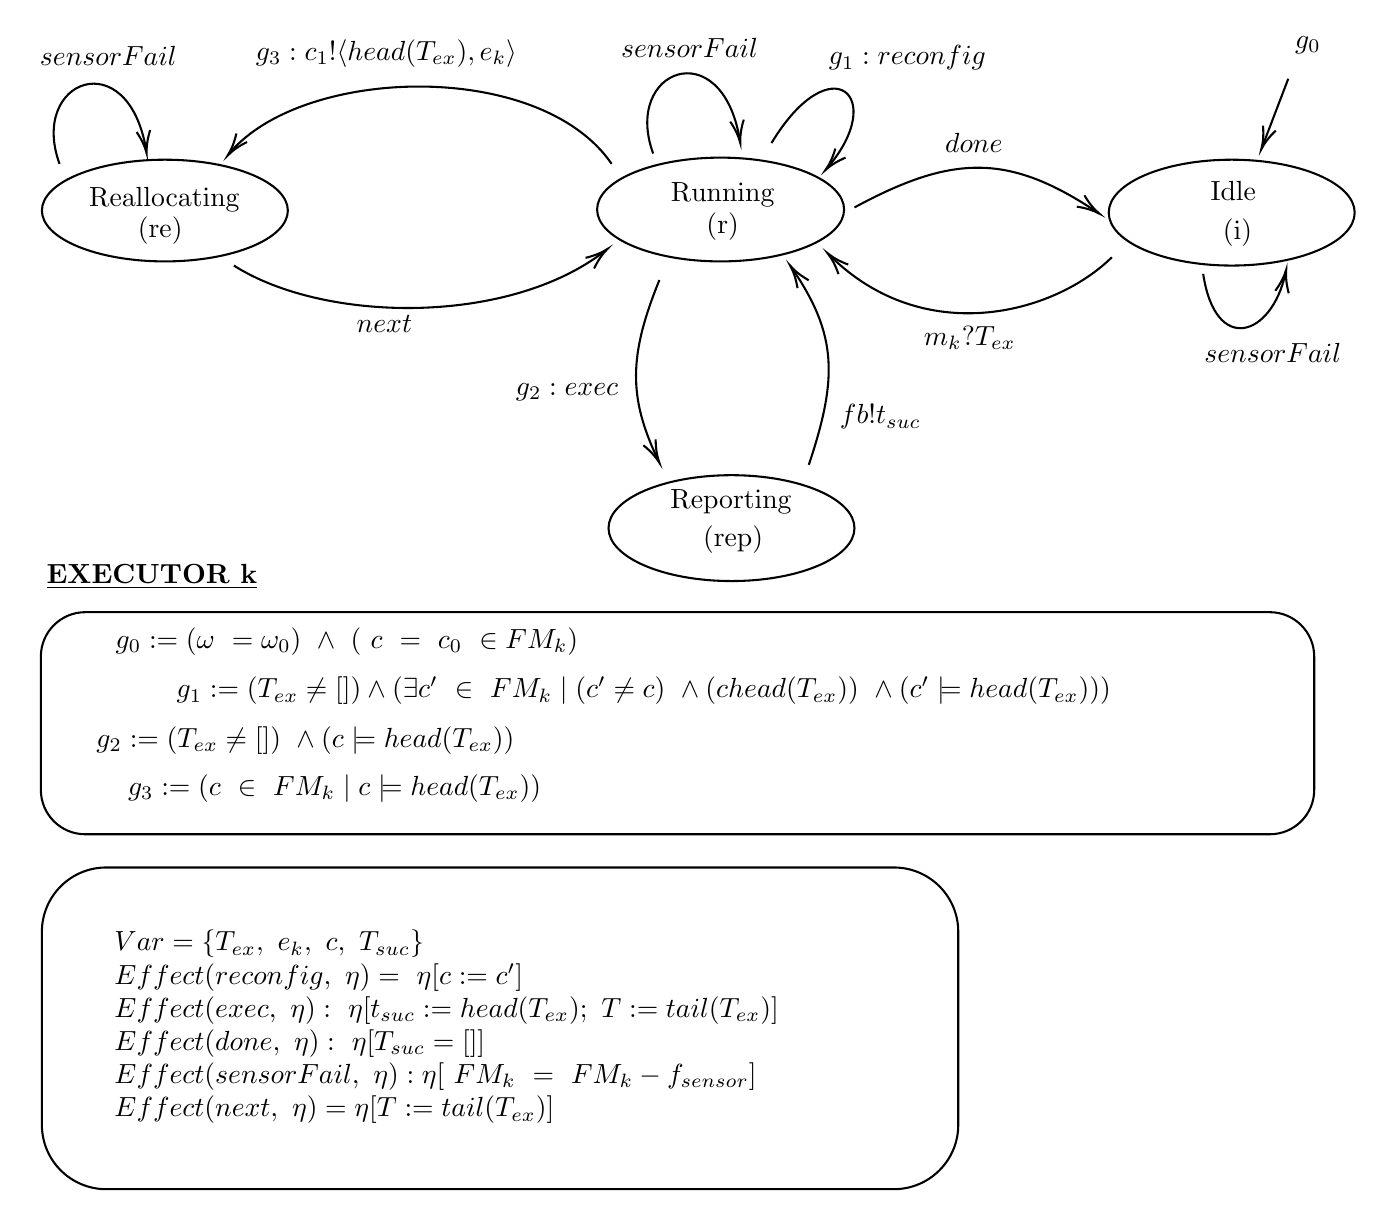
\begin{tikzpicture}[x=0.75pt,y=0.75pt,yscale=-1,xscale=1]
%uncomment if require: \path (0,582); %set diagram left start at 0, and has height of 582

%Curve Lines [id:da9480858267519683] 
\draw    (385.5,222) .. controls (399.29,180.63) and (399.5,159.63) .. (377.52,127.48) ;
\draw [shift={(376.5,126)}, rotate = 415.12] [color={rgb, 255:red, 0; green, 0; blue, 0 }  ][line width=0.75]    (10.93,-3.29) .. controls (6.95,-1.4) and (3.31,-0.3) .. (0,0) .. controls (3.31,0.3) and (6.95,1.4) .. (10.93,3.29)   ;
%Shape: Ellipse [id:dp6594609066072359] 
\draw   (283.5,99) .. controls (283.5,85.19) and (310.14,74) .. (343,74) .. controls (375.86,74) and (402.5,85.19) .. (402.5,99) .. controls (402.5,112.81) and (375.86,124) .. (343,124) .. controls (310.14,124) and (283.5,112.81) .. (283.5,99) -- cycle ;
%Shape: Ellipse [id:dp873836537729809] 
\draw   (530,100.5) .. controls (530,86.42) and (556.53,75) .. (589.25,75) .. controls (621.97,75) and (648.5,86.42) .. (648.5,100.5) .. controls (648.5,114.58) and (621.97,126) .. (589.25,126) .. controls (556.53,126) and (530,114.58) .. (530,100.5) -- cycle ;
%Curve Lines [id:da21020703050779688] 
\draw    (367.5,67) .. controls (396.21,19.48) and (423.94,44.49) .. (394.41,78.95) ;
\draw [shift={(393.5,80)}, rotate = 311.53] [color={rgb, 255:red, 0; green, 0; blue, 0 }  ][line width=0.75]    (10.93,-3.29) .. controls (6.95,-1.4) and (3.31,-0.3) .. (0,0) .. controls (3.31,0.3) and (6.95,1.4) .. (10.93,3.29)   ;
%Straight Lines [id:da37650774099478246] 
\draw    (616.5,36) -- (604.21,68.13) ;
\draw [shift={(603.5,70)}, rotate = 290.92] [color={rgb, 255:red, 0; green, 0; blue, 0 }  ][line width=0.75]    (10.93,-3.29) .. controls (6.95,-1.4) and (3.31,-0.3) .. (0,0) .. controls (3.31,0.3) and (6.95,1.4) .. (10.93,3.29)   ;
%Shape: Ellipse [id:dp02234558999259495] 
\draw   (16,99.5) .. controls (16,85.97) and (42.53,75) .. (75.25,75) .. controls (107.97,75) and (134.5,85.97) .. (134.5,99.5) .. controls (134.5,113.03) and (107.97,124) .. (75.25,124) .. controls (42.53,124) and (16,113.03) .. (16,99.5) -- cycle ;
%Curve Lines [id:da2517277021570281] 
\draw    (290.5,77) .. controls (255.85,26.51) and (141.81,29.93) .. (106.54,71.72) ;
\draw [shift={(105.5,73)}, rotate = 308.33000000000004] [color={rgb, 255:red, 0; green, 0; blue, 0 }  ][line width=0.75]    (10.93,-3.29) .. controls (6.95,-1.4) and (3.31,-0.3) .. (0,0) .. controls (3.31,0.3) and (6.95,1.4) .. (10.93,3.29)   ;
%Curve Lines [id:da851947022127026] 
\draw    (108.5,126) .. controls (152.06,153.72) and (240.7,154.98) .. (287.11,119.1) ;
\draw [shift={(288.5,118)}, rotate = 501.19] [color={rgb, 255:red, 0; green, 0; blue, 0 }  ][line width=0.75]    (10.93,-3.29) .. controls (6.95,-1.4) and (3.31,-0.3) .. (0,0) .. controls (3.31,0.3) and (6.95,1.4) .. (10.93,3.29)   ;
%Curve Lines [id:da05773774536505705] 
\draw    (531.5,122) .. controls (503.29,149.72) and (440.77,165.68) .. (395.86,121.36) ;
\draw [shift={(394.5,120)}, rotate = 405.63] [color={rgb, 255:red, 0; green, 0; blue, 0 }  ][line width=0.75]    (10.93,-3.29) .. controls (6.95,-1.4) and (3.31,-0.3) .. (0,0) .. controls (3.31,0.3) and (6.95,1.4) .. (10.93,3.29)   ;
%Rounded Rect [id:dp5913972444482631] 
\draw   (15.5,314.4) .. controls (15.5,302.58) and (25.08,293) .. (36.9,293) -- (607.6,293) .. controls (619.42,293) and (629,302.58) .. (629,314.4) -- (629,378.6) .. controls (629,390.42) and (619.42,400) .. (607.6,400) -- (36.9,400) .. controls (25.08,400) and (15.5,390.42) .. (15.5,378.6) -- cycle ;
%Rounded Rect [id:dp9206164489184118] 
\draw   (16,447) .. controls (16,429.88) and (29.88,416) .. (47,416) -- (426.5,416) .. controls (443.62,416) and (457.5,429.88) .. (457.5,447) -- (457.5,540) .. controls (457.5,557.12) and (443.62,571) .. (426.5,571) -- (47,571) .. controls (29.88,571) and (16,557.12) .. (16,540) -- cycle ;
%Curve Lines [id:da46585089178877326] 
\draw    (24.5,77) .. controls (9.65,36.41) and (57.53,18.36) .. (66.25,70.4) ;
\draw [shift={(66.5,72)}, rotate = 261.57] [color={rgb, 255:red, 0; green, 0; blue, 0 }  ][line width=0.75]    (10.93,-3.29) .. controls (6.95,-1.4) and (3.31,-0.3) .. (0,0) .. controls (3.31,0.3) and (6.95,1.4) .. (10.93,3.29)   ;
%Curve Lines [id:da24525569786800605] 
\draw    (575.5,130) .. controls (581.38,169.2) and (608.39,160.38) .. (615.11,129.89) ;
\draw [shift={(615.5,128)}, rotate = 460.62] [color={rgb, 255:red, 0; green, 0; blue, 0 }  ][line width=0.75]    (10.93,-3.29) .. controls (6.95,-1.4) and (3.31,-0.3) .. (0,0) .. controls (3.31,0.3) and (6.95,1.4) .. (10.93,3.29)   ;
%Curve Lines [id:da5617910694928671] 
\draw    (310.5,72) .. controls (295.65,31.41) and (343.53,13.36) .. (352.25,65.4) ;
\draw [shift={(352.5,67)}, rotate = 261.57] [color={rgb, 255:red, 0; green, 0; blue, 0 }  ][line width=0.75]    (10.93,-3.29) .. controls (6.95,-1.4) and (3.31,-0.3) .. (0,0) .. controls (3.31,0.3) and (6.95,1.4) .. (10.93,3.29)   ;
%Shape: Ellipse [id:dp893416141673501] 
\draw   (289,252.5) .. controls (289,238.42) and (315.53,227) .. (348.25,227) .. controls (380.97,227) and (407.5,238.42) .. (407.5,252.5) .. controls (407.5,266.58) and (380.97,278) .. (348.25,278) .. controls (315.53,278) and (289,266.58) .. (289,252.5) -- cycle ;
%Curve Lines [id:da2982425830385871] 
\draw    (313.5,133) .. controls (298.72,169.45) and (298.5,189.4) .. (312.84,219.61) ;
\draw [shift={(313.5,221)}, rotate = 244.18] [color={rgb, 255:red, 0; green, 0; blue, 0 }  ][line width=0.75]    (10.93,-3.29) .. controls (6.95,-1.4) and (3.31,-0.3) .. (0,0) .. controls (3.31,0.3) and (6.95,1.4) .. (10.93,3.29)   ;
%Curve Lines [id:da08998093824564413] 
\draw    (407.5,98) .. controls (455.02,72.26) and (481.96,72) .. (524.21,100.14) ;
\draw [shift={(525.5,101)}, rotate = 214] [color={rgb, 255:red, 0; green, 0; blue, 0 }  ][line width=0.75]    (10.93,-3.29) .. controls (6.95,-1.4) and (3.31,-0.3) .. (0,0) .. controls (3.31,0.3) and (6.95,1.4) .. (10.93,3.29)   ;

% Text Node
\draw (344,92) node   [align=left] {Running};
% Text Node
\draw (590,90) node   [align=left] {Idle};
% Text Node
\draw (420,199) node    {$fb!t_{suc}$};
% Text Node
\draw (182,24) node    {$g_{3} :c_{1} !\langle head( T_{ex}) ,e_{k} \rangle $};
% Text Node
\draw (463,161) node    {$m_{k} ?T_{ex}$};
% Text Node
\draw (75,94) node   [align=left] {Reallocating};
% Text Node
\draw (181,154) node    {$next$};
% Text Node
\draw (306,331) node    {$g_{1} :=( T_{ex} \neq []) \land ( \exists c'\ \in \ \llbracket FM_{k} \rrbracket \mid ( c'\neq c) \ \land ( c\nvDash head( T_{ex})) \ \land ( c'\models head( T_{ex})))$};
% Text Node
\draw (433,26) node    {$g_{1} :reconfig$};
% Text Node
\draw (269,187) node    {$g_{2} :exec$};
% Text Node
\draw (143,355) node    {$g_{2} :=( T_{ex} \neq []) \ \land ( c\models head( T_{ex}))$};
% Text Node
\draw (152,461) node    {$ \begin{array}{l}
\end{array}$};
% Text Node
\draw (211,493) node    {$ \begin{array}{l}
Var=\{T_{ex} ,\ e_{k} ,\ c,\ T_{suc}\}\\
Effect( reconfig,\ \eta ) =\ \eta [ c:=c']\\
Effect( exec,\ \eta ) :\ \eta [ t_{suc} :=head( T_{ex}) ;\ T:=tail( T_{ex})]\\
Effect( done,\ \eta ) :\ \eta [ T_{suc} =[]]\\
Effect( sensorFail,\ \eta ) :\eta [ \ FM_{k} \ =\ FM_{k} -f_{sensor}]\\
Effect( next,\ \eta ) =\eta [ T:=tail( T_{ex})]
\end{array}$};
% Text Node
\draw (73,109) node   [align=left] {(re)};
% Text Node
\draw (344,107) node   [align=left] {(r)};
% Text Node
\draw (592,110) node   [align=left] {(i)};
% Text Node
\draw (626,20) node    {$g_{0}$};
% Text Node
\draw (157,378) node    {$g_{3} :=( \nexists c\ \in \ \llbracket FM_{k} \rrbracket \mid c\models head( T_{ex}))$};
% Text Node
\draw (163,307) node    {$g_{0} :=( \omega \ =\omega _{0}) \ \land \ ( \ c\ =\ c_{0} \ \in \llbracket FM_{k} \rrbracket )$};
% Text Node
\draw (48,25) node    {$sensorFail$};
% Text Node
\draw (609,168) node    {$sensorFail$};
% Text Node
\draw (465,67) node    {$done$};
% Text Node
\draw (328,21) node    {$sensorFail$};
% Text Node
\draw (348,240) node   [align=left] {Reporting};
% Text Node
\draw (349,258) node   [align=left] {(rep)};
% Text Node
\draw (69,276) node   [align=left] {\textbf{\underline{EXECUTOR k}}};


\end{tikzpicture}
\label{executor}
\caption{Task Executor PG to an element $e_k$}
\end{figure}
